%% Copyright (C) 2018 Adrien Blanchet
%%

%%%%%%%%%%%%%%%%%%%%%%%%%%%%%%%%%%%%%%%%
%             Chapitre Simulation               %
%%%%%%%%%%%%%%%%%%%%%%%%%%%%%%%%%%%%%%%%

\chapter{Simulation de \textsc{Stereo}}
\label{chap:chapitre_3}

\citationChap{
On the other side of the screen, it all looks so easy!
}{Kevin Flynn}{Tron (1982)}

\minitoc

\newpage

\lettrine{À}{} l'instar de la révolution qu'a subit l'astrophysique au début du XXIe siècle grâce au développement des technologies embarquées à bord des satellites, les progrès en informatique, logiciels et matériels, ont véritablement transformé l'approche empruntée par les scientifiques pour comparer des données avec des modèles prédictifs. Aujourd'hui les expériences menées en physique des particules, et plus généralement en physique fondamentale, reposent sur un aspect tout aussi crucial que l'instrumentation : la simulation. La géométrie des détecteurs ainsi que les exigences sur la précision des mesures requièrent souvent une grande maitrise de l'ensemble des processus physiques qui engendrent le signal qui est interprété. La simulation, terme souvent substitué par \og Monte-Carlo \fg{}, est d'un enjeu primordial en vertu de la pertinence des résultats de physiques que prétend apporter une expérience. Cet aspect s'est naturellement imposé aux physiciens à mesure que le poids (financier) des projets expérimentaux a cru jusqu'à ce que le principe de reproductivité, sur lequel repose la méthode scientifique, s'est presque retrouvé compromis. En d'autres termes : aujourd'hui la validité de chaque mesure est capitale. Pour palier à ce nouveau défi, les scientifiques ont couplés les avancées dans le domaine de la simulation du transport de particules dans un milieu, avec des méthodes statistiques tout droit sorties de la culture des mathématiciens. Comme son nom l'indique, ce chapitre est consacré à la simulation de l'instrumentation de \textsc{Stereo} et constitue l'effort de travail principal auquel s'est attelé la collaboration dans le cadre de l'analyse de données. L'enjeu est de taille en effet, car c'est cette simulation qui est en charge de générer les spectres positrons qui sont directement comparés aux données. Ce chapitre retrace donc les principaux aspects du Monte-Carlo depuis la propagation des particules dans le détecteur jusque la procédure de construction des spectres positrons tenant compte d'une oscillation vers un neutrino stérile.\\

\section{Le détecteur dans \textsc{Geant4}}

Les études sur le prototype de \textsc{Stereo} avaient montré que la réponse en énergie dépendait de deux principaux facteurs : les fuites d'énergie dues à la géométrie des cellules, et les inhomogénéités de collection de lumière dans le volume de détection  (\cite{bonhomme:tel-01931309}, chapitre 3). Les zones mortes du détecteur doivent donc être précisément modélisées afin de décrire correctement les quantités d'énergie véritablement déposées dans le volume actif. De plus, l'implémentation d'un modèle optique dans la simulation est nécessaire pour reproduire la forme des distributions de charges collectées par les PMs avec différentes configurations spatiales de dépôts en énergie. La maitrise de l'ensemble de ces phénomènes est capitale pour contraindre l'échelle en énergie sur toute la gamme du spectre neutrino ainsi que pour contrôler l'efficacité des coupures topologiques employées pour optimiser le rapport signal sur bruit. De ce constat est né le code de simulation dédié au détecteur \textsc{Stereo}.\\

Le code de simulation par méthode Monte-Carlo (MC) est mis à disposition dans un répertoire commun à la collaboration, où chaque version est archivée à l'aide d'\textit{Apache Subversion} (svn)\footnote{\url{https://svn.in2p3.fr/stereo/}}. Le c\oe ur de la simulation est basé sur les bibliothèques C++ \textsc{Geant4} \cite{Agostinelli:2002hh} destinées à simuler le passage de particules au travers la matière. Cette boite à outils permet de simuler divers processus physiques (électromagnétiques, hadroniques et optiques) sur une gamme d'énergies allant de quelques centaines d'eV jusqu'au TeV, tout en tenant compte de la géométrie des détecteurs et de la composition des matériaux. D'autre part, le code de simulation \textsc{Stereo} contient des éléments directement hérités de Double Chooz \cite{Abe:2014bwa}, qui eux-mêmes trouvent leur origine dans le code de simulation dédié à KamLAND (\textit{GLG4sim}) \cite{Smith:2005}. Cet héritage procure l'ensemble des avancements acquis durant les deux dernières décennies sur la simulation des détecteurs neutrinos exploitant des liquides scintillateurs. En effet, les phénomènes tels que l'émission de lumière par le processus de scintillation, sa conversion vers le domaine de sensibilité en longueur d'onde des PM, sa propagation optique, le \textit{quenching}, la PSD, l'émission de lumière par effet Cherenkov, ou encore la cascade de décroissance du Gadolinium sont traités et prêts à l'emploi. De plus, la géométrie et la réponse des photomultiplicateurs sont incluses dans \textit{GLG4sim} et seuls quelques paramètres physiques sont ajustés pour correspondre au cas de \textsc{Stereo}.\\

La forme de la réponse en énergie du détecteur \textsc{Stereo} est sensible à la géométrie du volume de détection. La structure en acrylique a donc été reproduite sur la base des plans de construction du détecteur\footnote{\url{http://dappcf9/Caomeca/Projet.php?proj=STEREO&mod=x&spr=x&sse=x}}, et le maximum de détails sur les bords, languettes, etc., a été pris en compte: voir Figures \ref{fig:geom_design} et \ref{fig:geom_G4}. Les buffers, les photomultiplicateurs ainsi que les tubes de calibrations sont aussi implémentés à partir des plans. Une vue de dessus du détecteur sur la figure \ref{fig:convention_axe_MC.png} montre la convention choisie pour les axes XYZ, ainsi que la numérotation des cellules.\\

La cuve en acier inoxydable qui contient la structure en acrylique est aussi incluse dans la simulation, de même que les différents blindages autour du détecteur. Ces éléments permettent d'étudier le taux de pénétration des bruits de fond dans la casemate. Afin d'étudier en particulier les bruits de fond d'origine cosmique, le veto muon, le canal de transfert ainsi que les blindages extérieurs jonchant les murs de séparation de la casemate avec les expériences voisines sont inclus.\\

\afterpage{

\begin{figure}[h!]
\centering
\begin{subfigure}[b]{0.49\textwidth}

\centering
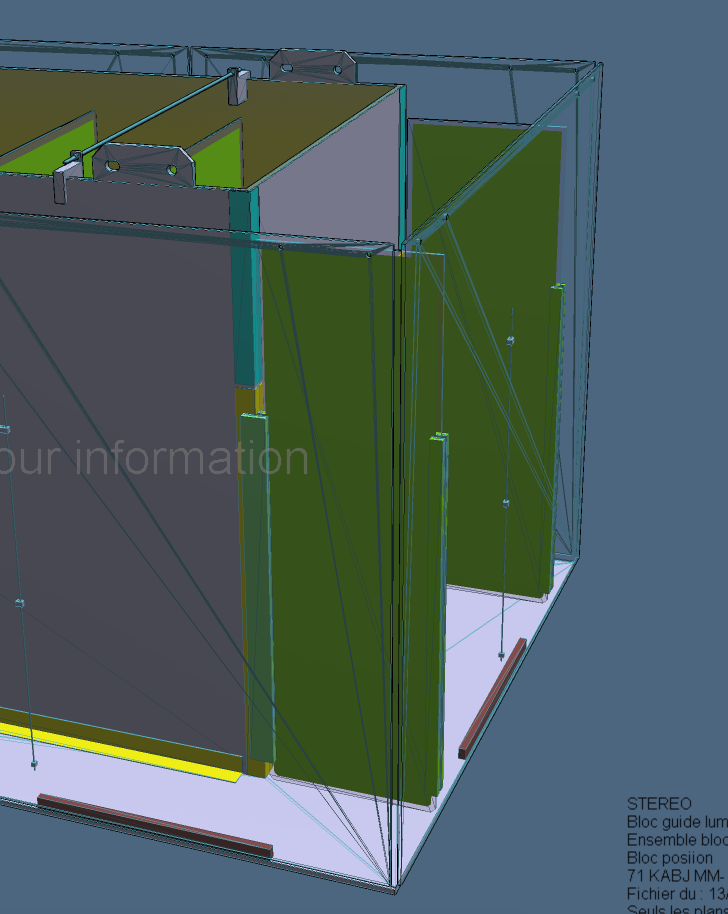
\includegraphics[height=0.3\paperheight]{images/geom_design2.png}
\captionof{figure}{}
\label{fig:geom_design}

\end{subfigure}
~ % attention ! space sensitive
\begin{subfigure}[b]{0.49\textwidth}

\centering
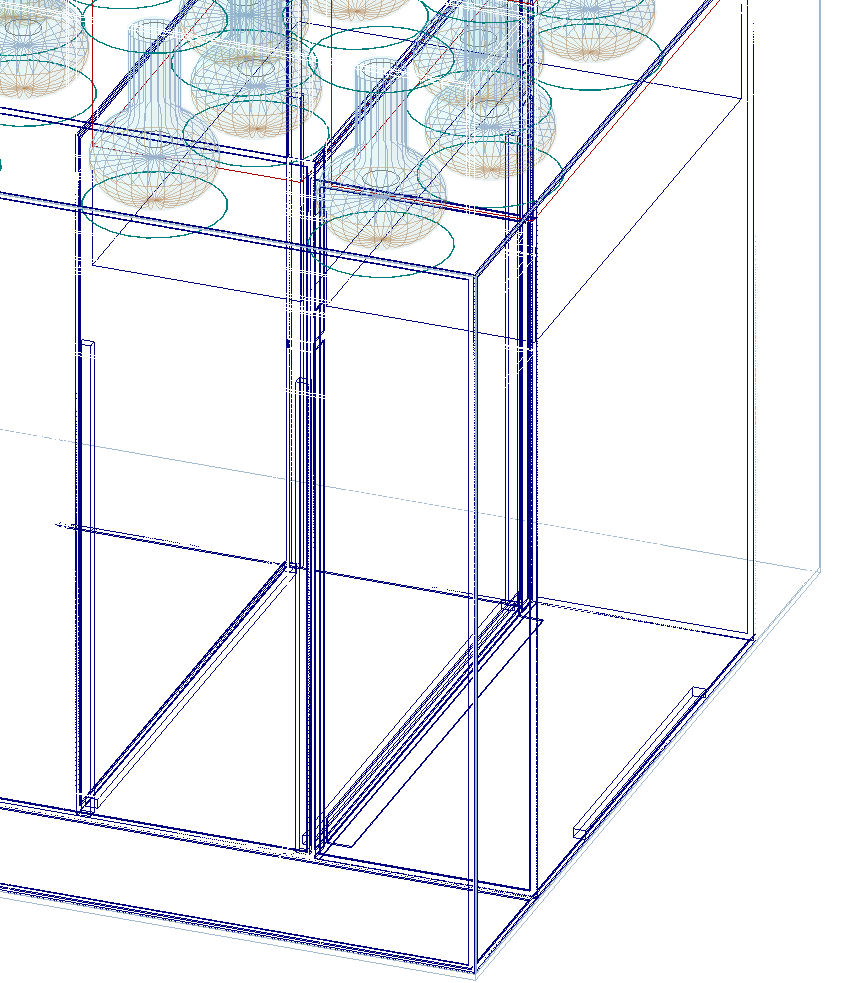
\includegraphics[height=0.3\paperheight]{images/geom_g4.png}
\captionof{figure}{}
\label{fig:geom_G4}

\end{subfigure}
%\captionof{figure}{Test}
\caption{Comparaison des détails fins de la géométrie interne du détecteur tels que décrits par le bureau d'étude (a) et \textsc{Geant4} (b).}
\label{fig:geom_comparison}
\end{figure}


\begin{figure}[h!]
\centering
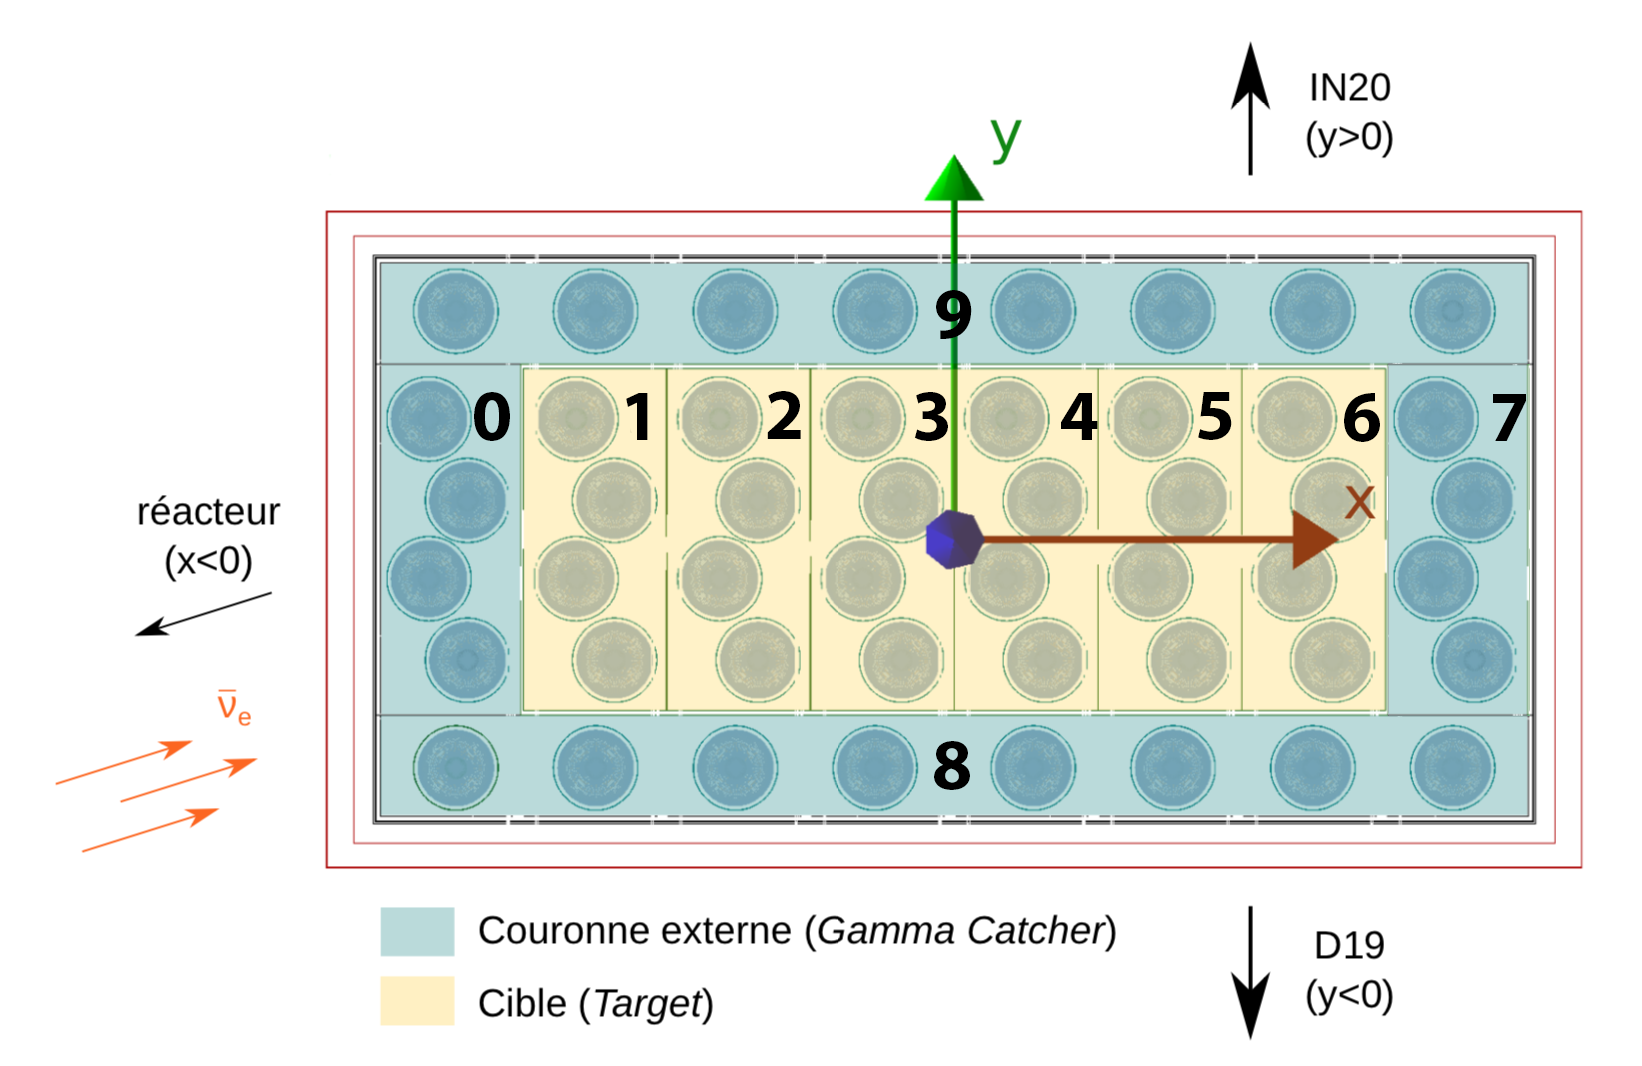
\includegraphics[width=1\linewidth]{images/convention_axe_MC.png}
\caption[Convention des axes dans la simulation et numérotation des cellules]{Convention des axes dans la simulation et numérotation des cellules. Les cellules de la Target sont numérotées de 1 à 6 tandis que les  cellules du Gamma-Catcher: 0, 7, 8 et 9. Le repère est placé au centre de la structure du détecteur interne. Chaque cercle correspond à un photomultiplicateur.}
\label{fig:convention_axe_MC.png}
\end{figure}

\clearpage

}


% Le code de simulation est à l'origine hérité de l'expérience NUCIFER,

\bigbreak

%\begin{itemize}
%    \item héritage code simu
%    \item structure acrylique
%\end{itemize}

\subsection{Simulation du passage d'une particule dans le détecteur}

\bigbreak

La simulation \textsc{Stereo} se sert directement des bibliothèques \textsc{Geant4} pour prendre en compte les interactions des particules dans le volume du détecteur. Cependant, pour des raisons d'optimisation de temps de calcul, seules les bibliothèques \textsc{Geant4} dites de basse énergie sont sollicitées. Les processus inclus sont par exemple : l'ionisation électronique, l'annihilation électron-positron, les diffusions élastiques hadroniques ou encore la capture des neutrons.\\

Les particules lancées dans le MC sont traitées sous forme de traces par \textsc{Geant4} et leur interaction avec l'environnement est entreprise en pas réguliers, aussi appelés \og \textit{steps} \fg{}. Plus les steps sont courtes, plus la simulation est fidèle, mais les temps de calcul requis augmente. \textsc{Geant4} adapte automatiquement la longueur des pas en fonction du libre parcours moyen, qui est estimé via les sections efficaces d'interactions des processus physiques que va subir la particule. À chaque step, une technique MC est utilisée pour décider de l'interaction qui se produit éventuellement. À l'issue de la réaction choisie, l'état de la particule incidente est mis à jour (énergie, impulsion, nature...) et si la réaction le requiert, des particules filles sont stockées dans une pile en vue d'être simulées ultérieurement.\\

Un \og événement simulé \fg{} contient l'ensemble des informations depuis l'émission de la particule injectée jusqu'à la propagation de toutes les particules filles. Une option \texttt{DeferTrack} est implémentée pour définir la fenêtre temporelle maximale d'un événement. Si après ce laps de temps les particules ne sont pas toutes propagées, les informations qui suivent sont attribuées à un nouvel événement. En pratique cet intervalle temporel est ajusté pour correspondre à la fenêtre d'intégration d'un pulse issu d'un PM. Cette option permet notamment de séparer les signaux Prompt et Retardés et ainsi de traiter les données simulées de la même manière que les vraies données.\\

Finalement, les événements simulés sont stockés dans un fichier \texttt{ROOT} sous forme d'entrées d'un arbre (\texttt{TTree}), où les propriétés de chaque trace sont enregistrées. De ces entrées sont par exemple extraites la quantité d'énergie totale \og déposée \fg{} dans le liquide scintillateur : $E^\textrm{dep}$. Cette grandeur s'avère particulièrement importante lors de la procédure de reconstruction en énergie, décrite dans le Chapitre \ref{chap:chapitre_energie}.\\

\bigbreak

% \textit{Il faudrait quand même décrie succintement le modèle optique de la scintillation avec les ingrédients des spectres d'émission et des fluors qui décalent la longeur d'onde. Dire aussi un mot de la composition chimique qui permet de suivre au mieux la densité réelle de protons.}

\subsection{Simulation du liquide scintillateur}

\bigbreak

Bien que les processus de scintillation ne sont pas directement simulés à partir de l'excitation des liaisons $\pi$ (cf. section \ref{seq:scintillation}), la composition et densité atomique du liquide est précisément spécifiée dans la simulation. En effet, une telle implémentation permet de suivre au mieux la densité réelle de protons de \textsc{Stereo}. Les composantes du liquide scintillateur sont des molécules organiques essentiellement constituées de carbone et d'hydrogène et fournissent à elles seules l'essentiel des cibles de protons pour les neutrinos. De plus, puisque le liquide est dopé au Gadolinium, la fraction de captures des neutrons doit être bien décrite dans la simulation pour estimer correctement l'efficacité de détection (cf. section \ref{sec:neutrino_biases_eff}).\\

Le volume du liquide dans la simulation a été ajusté sur la mesure effectuée durant le remplissage. La fraction de masse hydrogène dans le MC s'est montré en accord avec la valeur mesurée dans les données : $f_H^{MC} = 11,43 \%$, à comparer avec $f_H^{Data} = 11,45 \pm 0,11 \%$ \cite{docdb929}.\\

\afterpage{

\begin{figure}
  \centering
  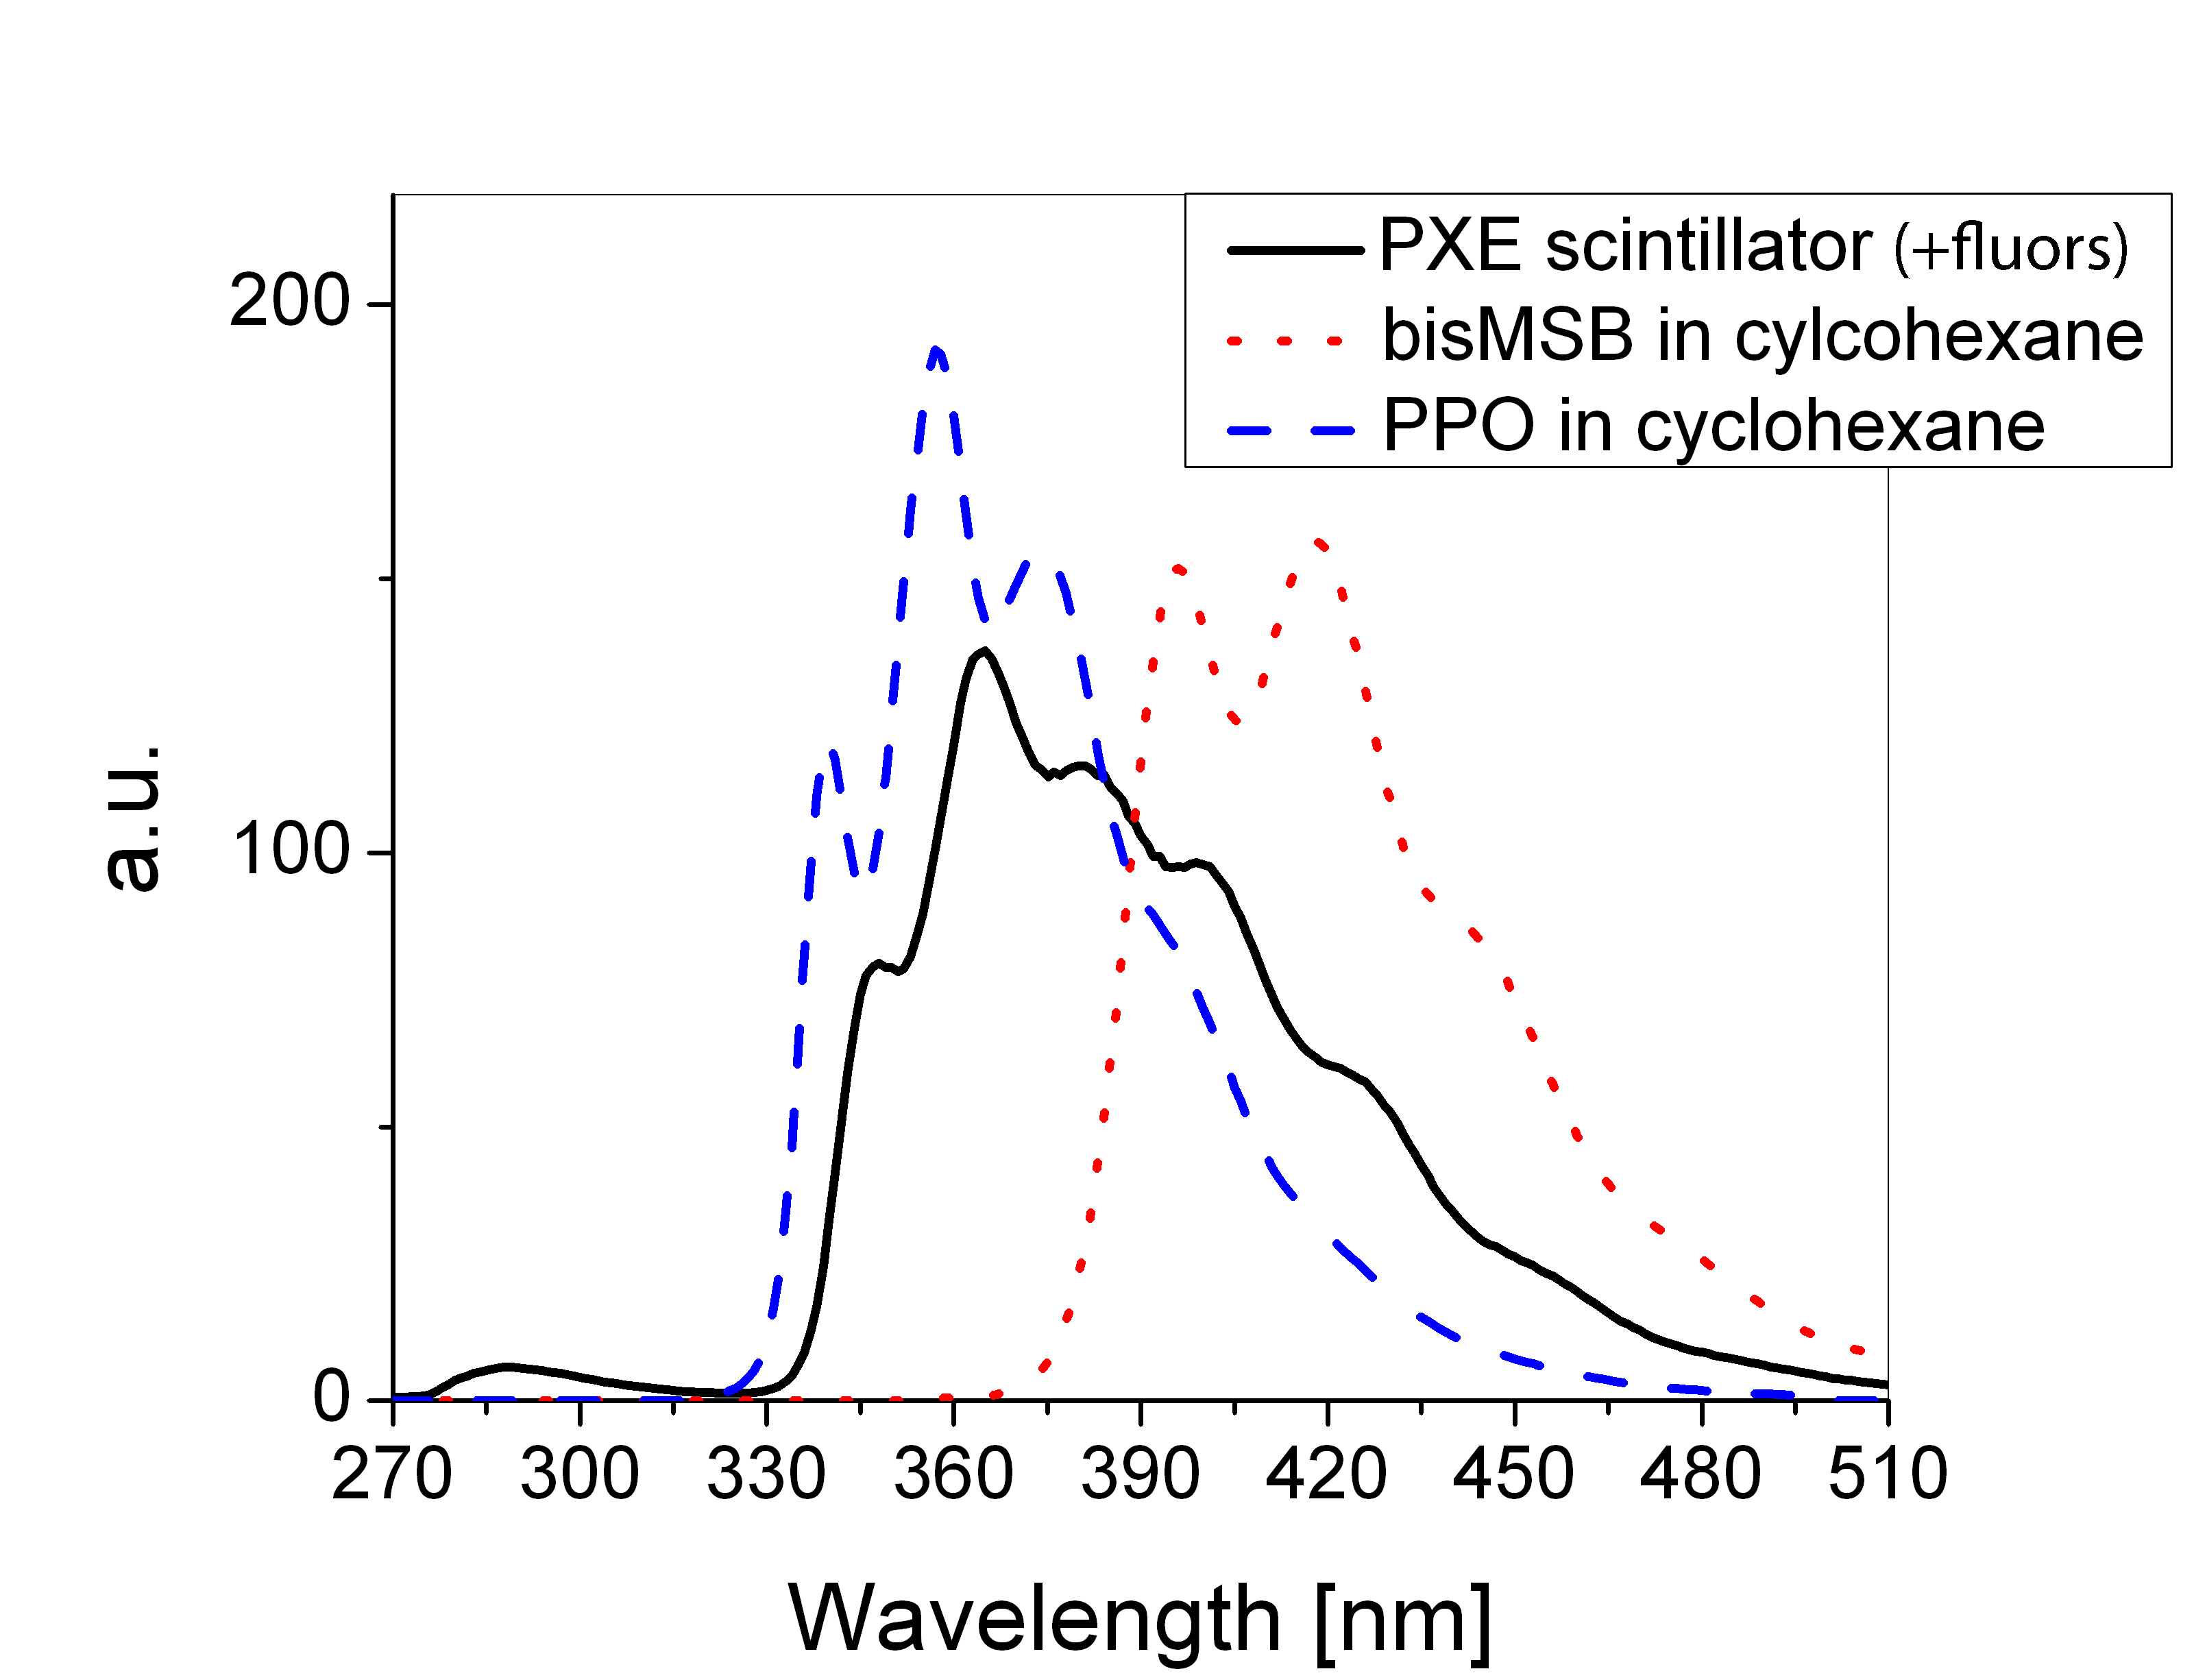
\includegraphics[width=0.8\linewidth]{images/fluore_spectrum.png}
  \caption[Spectres de réémission des photons par les fluores]{Spectres de réémission des photons par les fluores (noir). La courbe bleue représente le spectre de réémission du PPO seul et en rouge le spectre de réémission du bis-MSB. (source : \cite{Buck:2015jxa})}
  \label{fig:fluore_spectrum.png}
\end{figure}

}

La lumière de scintillation est émise photon par photon à chaque step \textsc{Geant4} suivant un spectre d'émission qui tient compte des wavelength shifters : PPO et Bis-MSB. En réalité, les photons émis qui circulent dans le liquide sont situés sur bande passante de longueurs d'onde entre $\SI{250}{nm}$ et $\SI{450}{nm}$. Lorsqu'ils sont absorbés par un atom de fluore (wavelength shifter), ils sont réémis suivant le spectre présenté sur la figure \ref{fig:fluore_spectrum.png}. C'est ce spectre qui est utilisé dans la simulation.\\

\afterpage{

\begin{figure}[h!]
\centering
\begin{subfigure}[b]{0.54\textwidth}

\centering
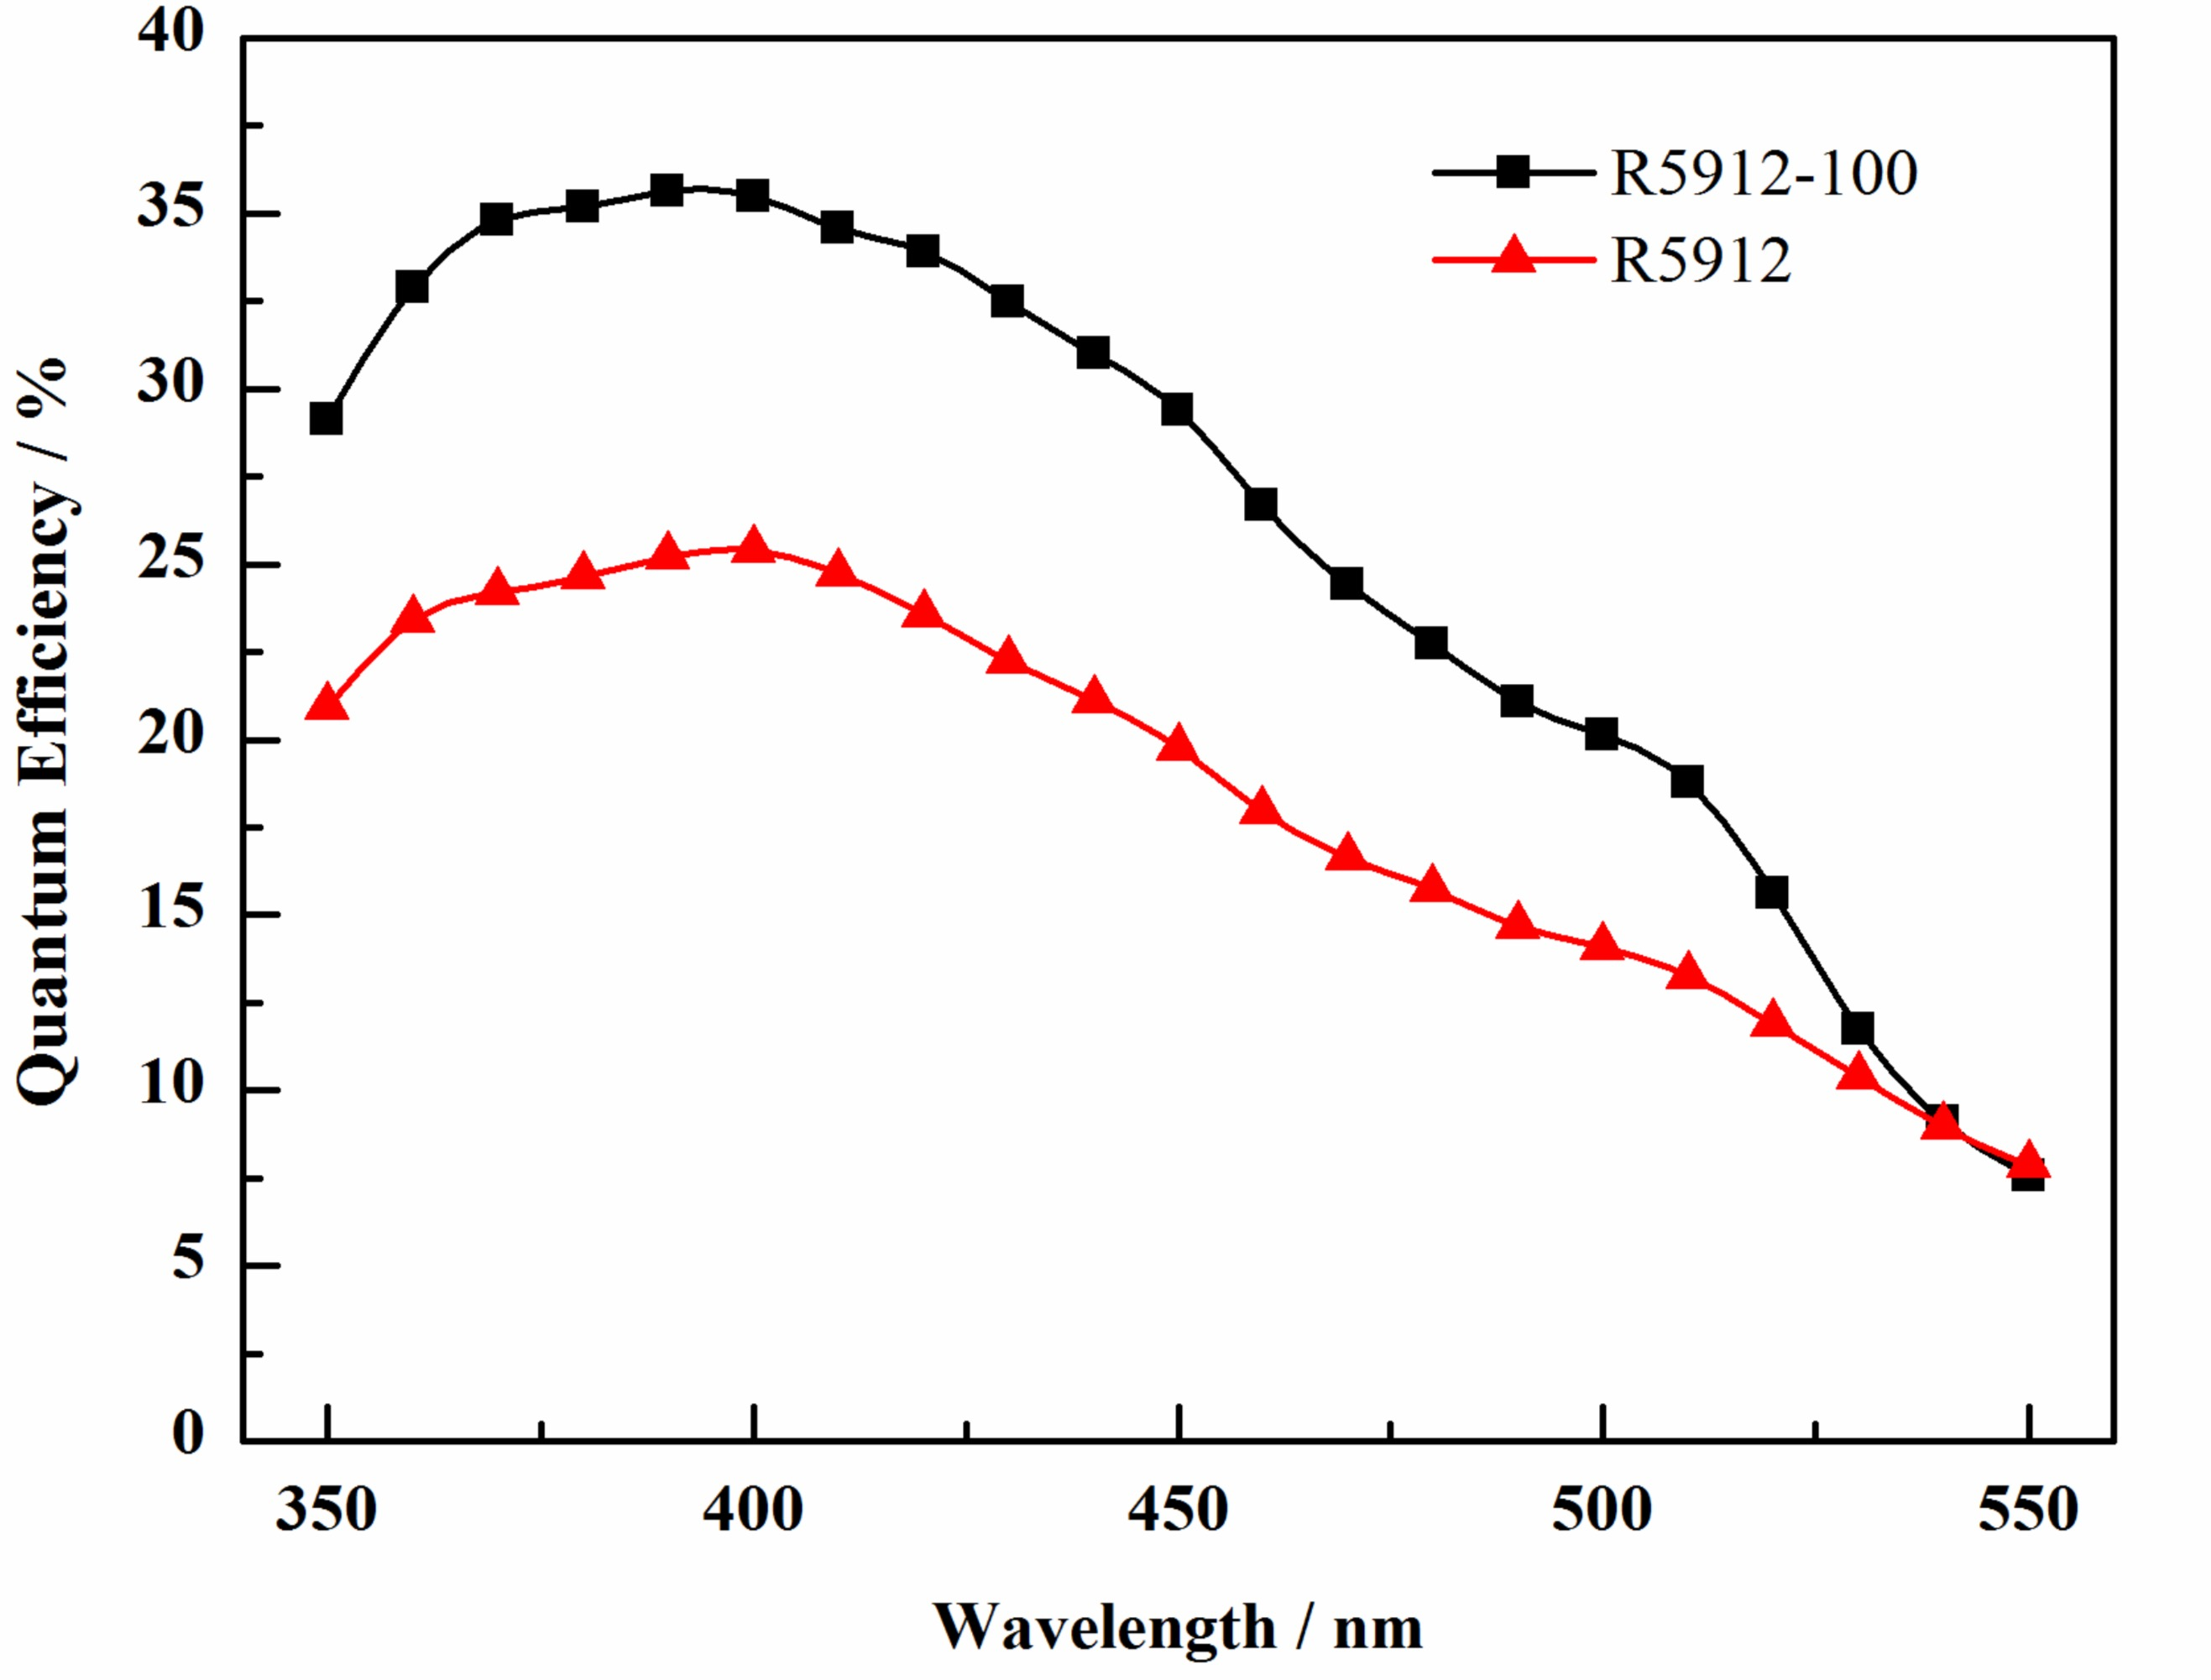
\includegraphics[width=1\textwidth]{images/wavelength_quantum_eff.jpg}
\caption{La courbe noire correspond aux PMs utilisés pour \textsc{Stereo}.}
\label{fig:wavelength_quantum_eff.jpg}

\end{subfigure}
~ % attention ! space sensitive
\begin{subfigure}[b]{0.44\textwidth}

\centering
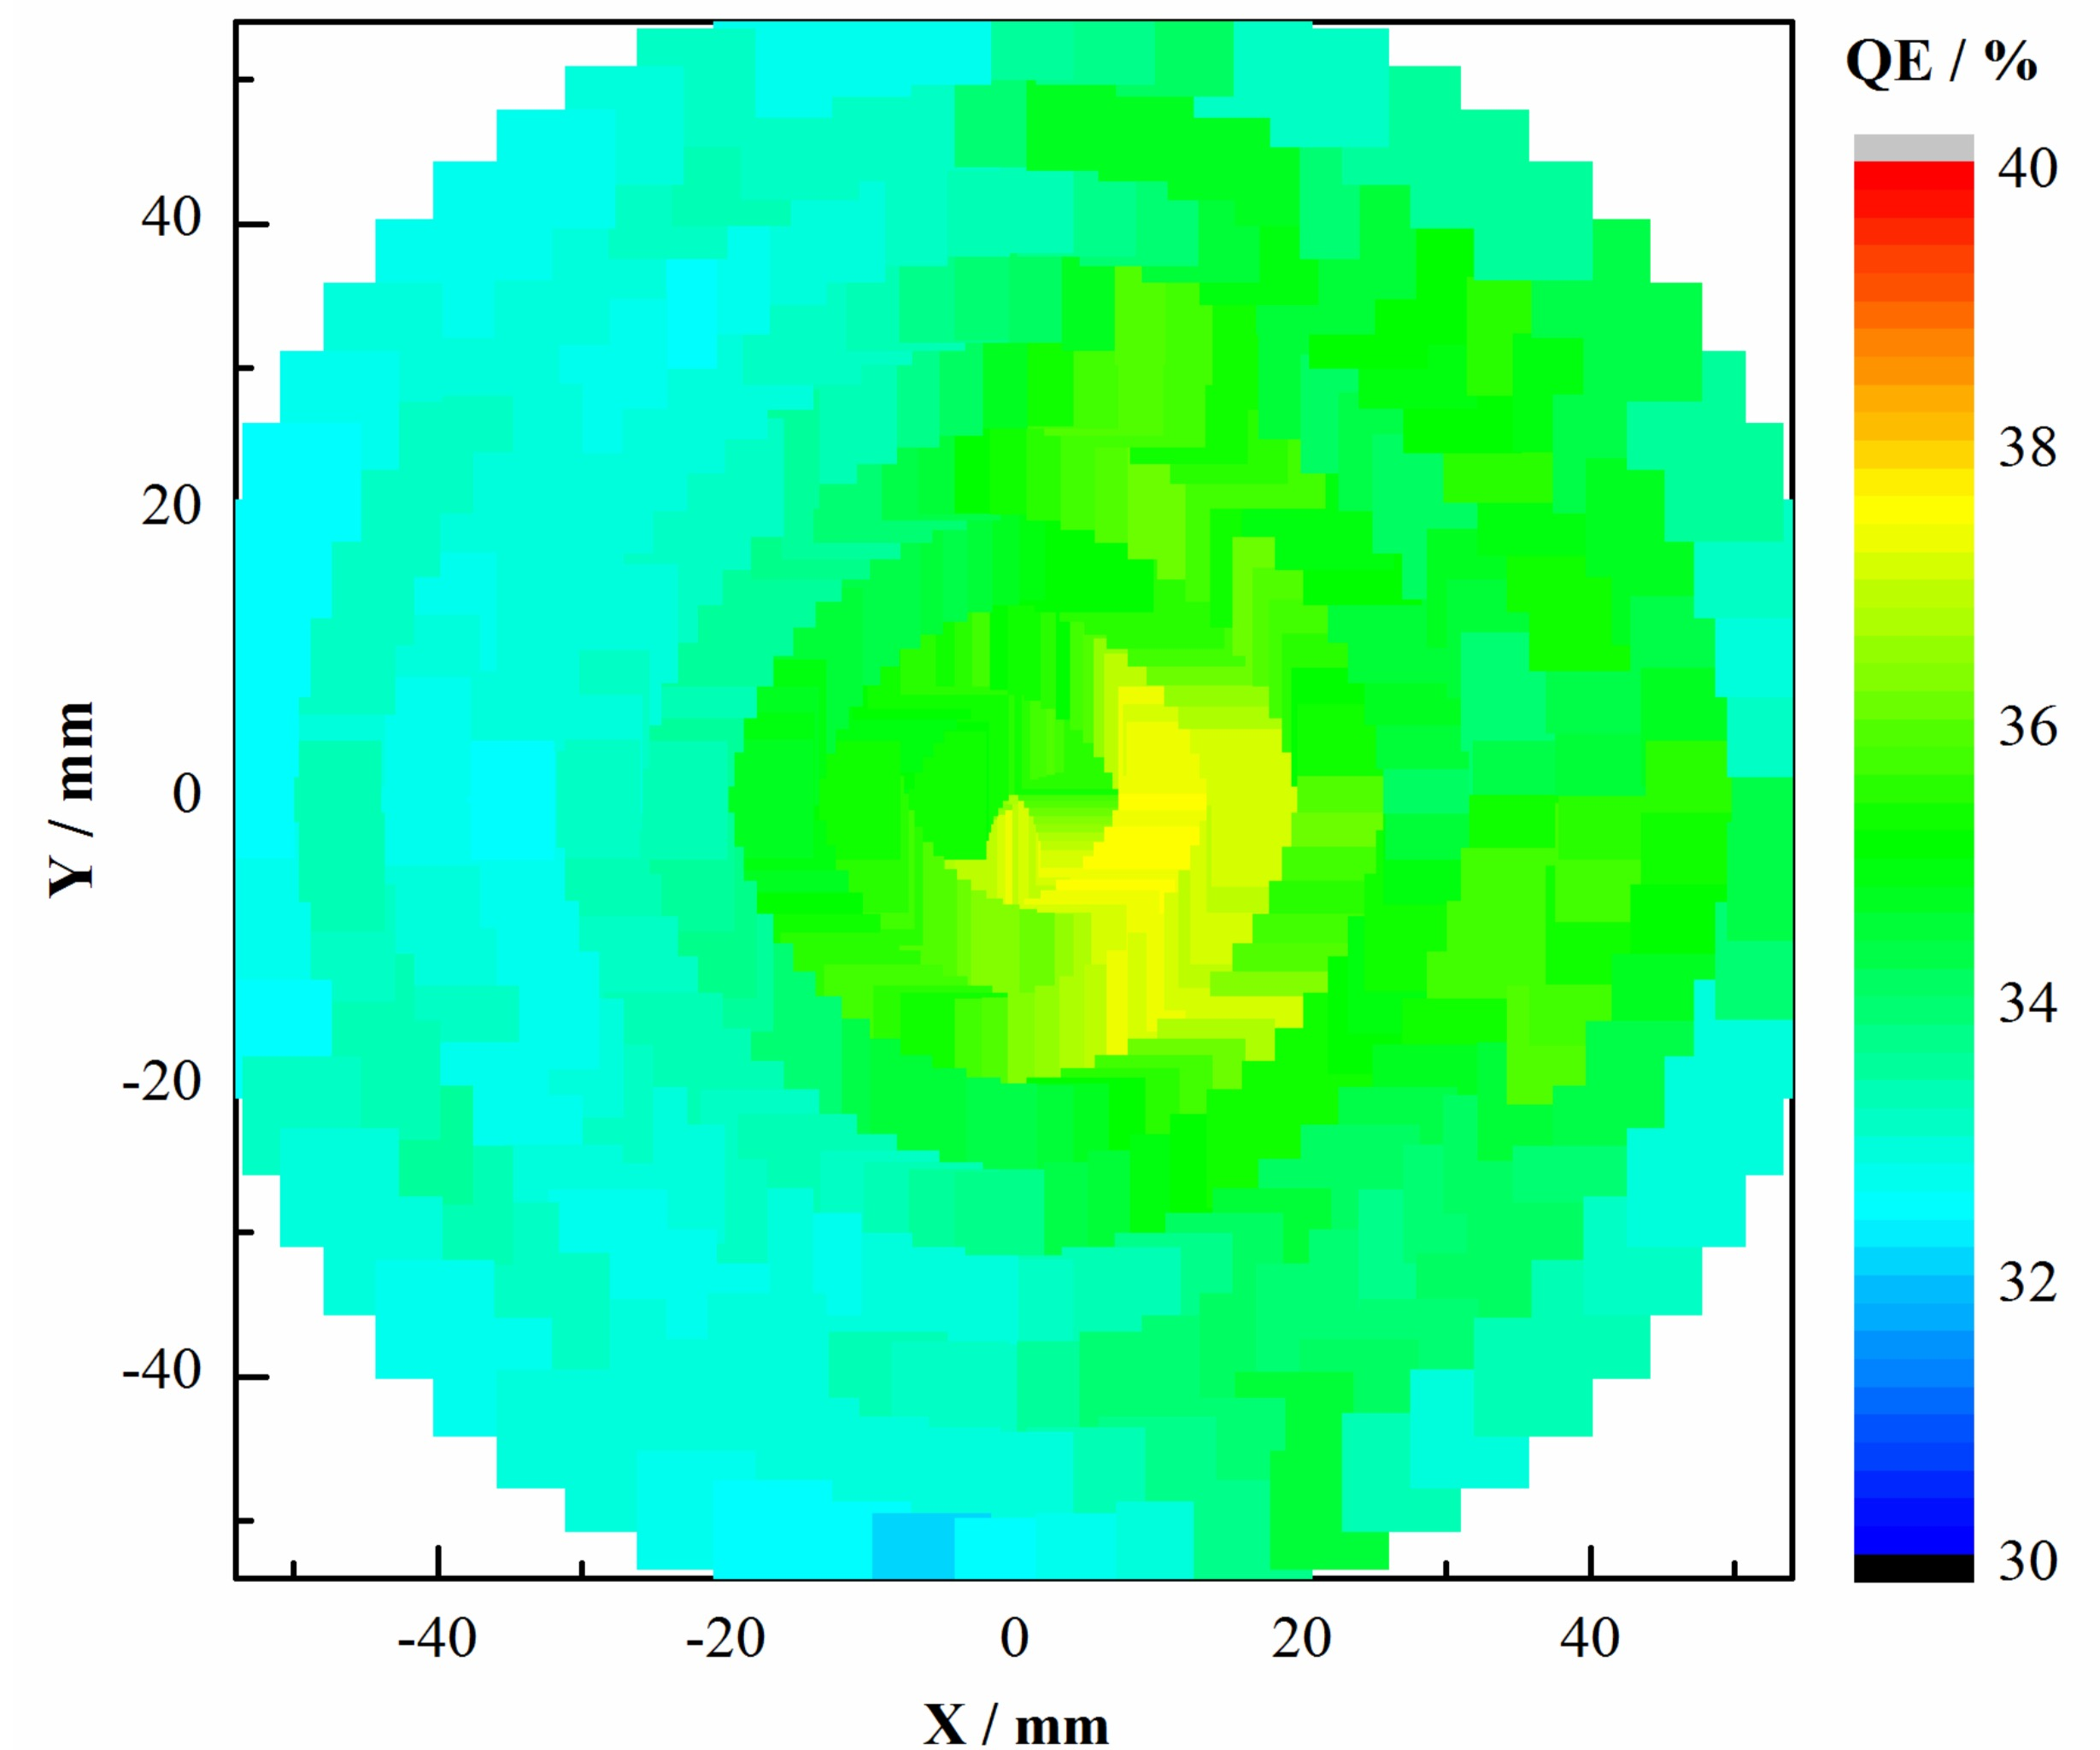
\includegraphics[width=1\textwidth]{images/position_dependant_quantum_eff.jpg}
\caption{}
\label{fig:position_dependant_quantum_eff.jpg}

\end{subfigure}
\caption[Dépendances de l'efficacité quantique des photomultiplicateurs]{Dépendances de l'efficacité quantique des photomultiplicateurs mesurés par \textsc{Wang} et al. \cite{Wang:2015vla}. L'efficacité quantique dépend de la longueur d'onde (a) ce qui justifie l'utilisation de fluores. L'efficacité de conversion dépend aussi de la position. }
\label{fig:PM_quantum_eff}
\end{figure}

}

Une fois émis, les photons optiques sont traqués par le moteur de la simulation jusqu'à leur disparition. Un photon subit une série d'absorptions-réémissions avant de disparaître une fois pour toutes. Cela arrive lorsqu'il est absorbé par une molécule, mais celle-ci se désexcite sans le réémettre: par exemple lorsqu'il est capturé par la photocathode d'un PM. La probabilité d'absorption est ajustée par la longueur d'atténuation qui est choisie pour correspondre avec la valeur mesurée en laboratoire. D'autre part, la conversion en photo-électron par les PMs est dirigée par l'efficacité quantique. Celle-ci a été mesurée en laboratoire par \textsc{Wang} et al. \cite{Wang:2015vla} en fonction de la longueur d'onde et de l'angle d'incidence du photon sur la photocathode (voir figure \ref{fig:PM_quantum_eff}). Ces dépendances de l'efficacité quantique sont implémentées dans le code de simulation \textsc{Stereo}.\\

Une fois l'ensemble des photons optiques traités, la chaine d'électronique est simulée et les données sont disposées dans un \texttt{TTree} ROOT estampillé \og Data \fg{}. Ce dernier a une structure identique à celui utilisé dans les véritables données. Ainsi, les études comparatives entre la simulation et les données sont établies avec les mêmes outils d'analyse.\\

\bigbreak

\subsection{Modèle optique des parois réfléchissantes}

Le modèle optique des parois réfléchissantes a été implémenté dans \textsc{Geant4} afin de reproduire au mieux les effets de volume sur la collection de lumière par les photomultiplicateurs. Un modèle effectif qui traite le sandwich en acrylique comme un unique matériau réfléchissant a été choisi afin de garder la flexibilité nécessaire lors de l'ajustement plus fin en comparant avec les vraies données du détecteur.\\

L'indice optique de l'acrylique est similaire à celui du liquide scintillateur. Les rayons lumineux traversent donc l'acrylique sans déviation jusqu'à atteindre le gap d'air qui précède le matériau réfléchissant (ESR). L'angle d'incidence critique entre l'air et l'acrylique est déterminé par $\theta_c = \textrm{arcsin}(n_{\textrm{air}}/n_{\textrm{acrylique}}) \sim 42^{\circ}$. Les rayons lumineux qui ont un angle d'incidence supérieur à $\theta_c$ sont réfléchis tandis que les autres sont transmis. Ces derniers finissent par atteindre la feuille réfléchissante dont la réflectivité avec l'air a été mesurée en fonction de la longueur d'onde. Ces différents cas sont représentés sur la figure \ref{fig:reflexion_process.png}.\\

\afterpage{

\begin{figure}
  \centering
  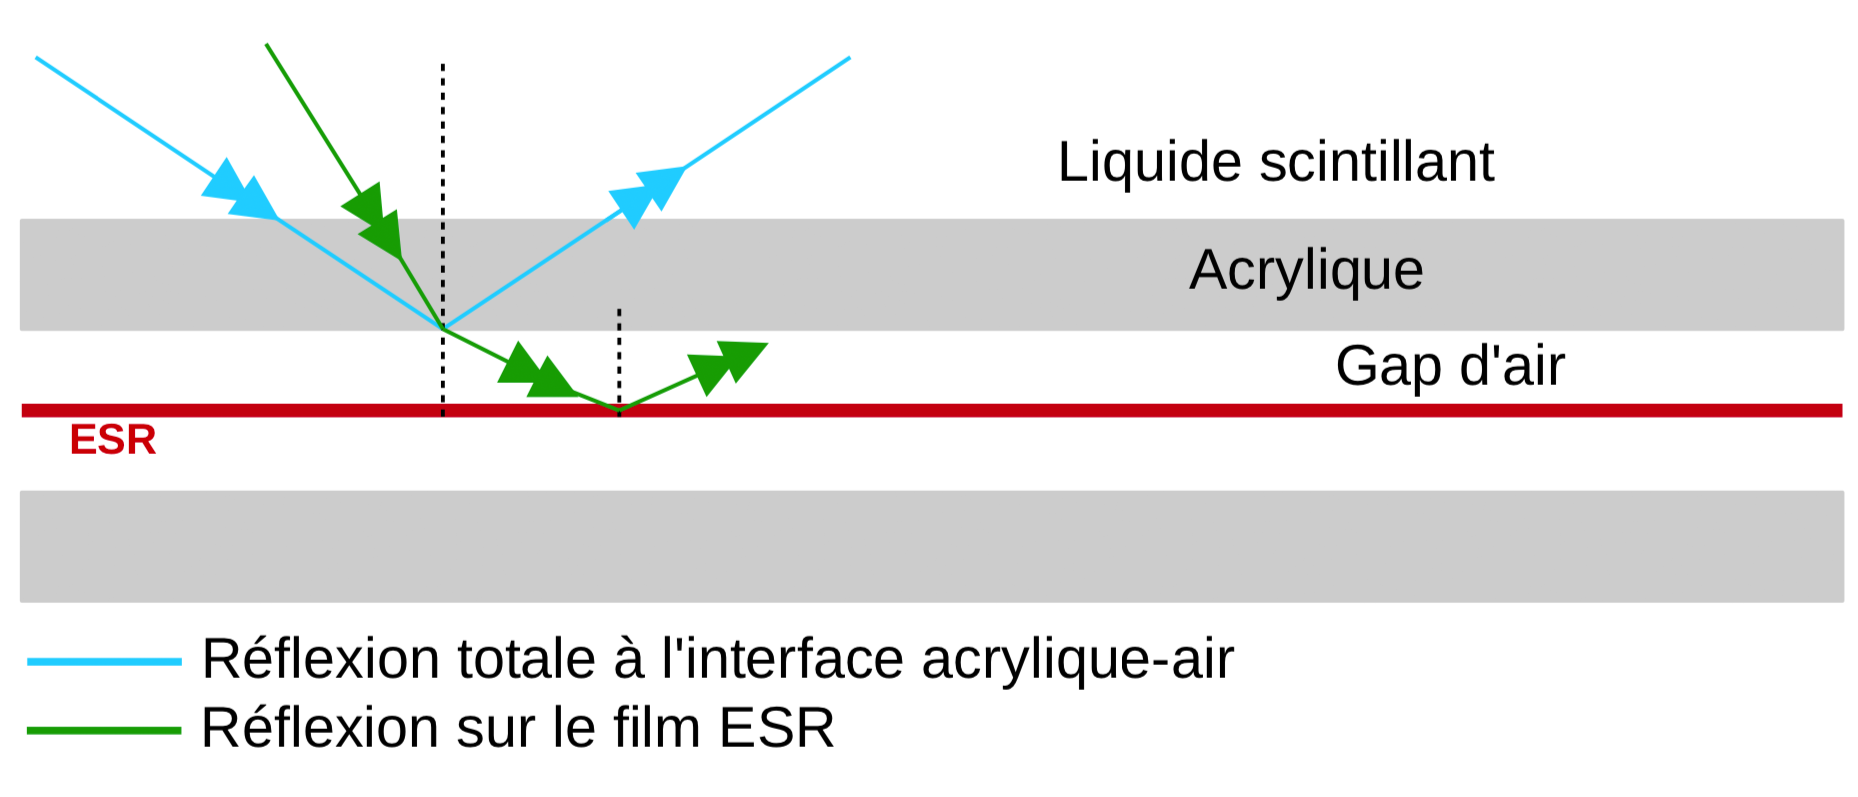
\includegraphics[width=0.7\linewidth]{images/reflexion_process.png}
  \caption[Représentation schématique d'un sandwich en acrylique]{Représentation schématique d'un sandwich en acrylique. Le sandwich maintient une feuille d'ESR dans l'air pour conserver ses propriétés optiques. La réflexion se produit soit à l'interface acrylique-air (rayon bleu), soit à l'interface air-ESR (rayon vert). (source : \cite{bonhomme:tel-01931309})}
  \label{fig:reflexion_process.png}
\end{figure}

}

Dans la simulation, un rayon qui atteint une paroi en acrylique est réfléchi avec une probabilité déterminée comme suit:\\

\begin{equation}
    R(\theta, \lambda) =
    \begin{cases}
        100\% & \text{, si } \theta > \theta_c\\
        R^{\text{ESR}}(\theta, \lambda) =
        \begin{cases}
            10 \%, & \text{si } \lambda < \SI{400}{nm}\\
            97 \%, & \text{si } \lambda > \SI{400}{nm}
        \end{cases}
        & \text{, sinon.}
    \end{cases}
\end{equation}

\bigbreak

Comme il a été décrit dans la section \ref{sec:assemblage}, la défaillance des joints de colle a laissé pénétrer le liquide scintillateur à l'intérieur de plusieurs sandwichs acryliques. Sans le contact avec le gap d'air, les propriétés réfléchissantes de l'ESR sont dégradées. Dans la simulation, le niveau d'infiltration du liquide à une hauteur $Z_c$ est ajusté pour chaque paroi. En dessous de $Z_c$ (là où le liquide a remplacé l'air), une coupure sur l'angle d'incidence est appliquée : $R(\theta, \lambda) = 0$ si $\theta \gtrsim \ang{70}$ \cite{docdb351}.\\

Les rayons lumineux qui ne sont pas réfléchis sont soit transmis, soit absorbés par le matériau. Des mesures avec le détecteur sans liquide scintillateur ont été menés afin d'estimer la part relative d'absorption et de transmission \cite{bonhomme:tel-01931309}. En comparant la lumière collectée par les cellules voisines, ces études ont montré que le terme d'absorption est très faible pour les cellules de la cible.\\

% Pour les fuites de lumières vers le Gamma Catcher cependant, la proportion est d'un 1/3 de transmission contre 2/3 d'absorption \cite{docdb151}.\\

\bigbreak

%\begin{itemize}
%    \item Coefficient de reflexion en fonction de l'angle / longueur d'onde
%    \item modèle effectif pour prendre en compte parois immergées
%\end{itemize}

\subsection{Ajustement sur les données}

La simulation est confrontée au véritable détecteur en comparant la réponse en charges collectées dans chaque cellule:

\begin{equation}
    Q_{i} = \sum_p^{\textrm{PM $\in$ cell $i$}} Q_{\text{tot}}^{p},
    \label{eq:qtot_cell}
\end{equation}

où $Q_i$ est le nombre de photo-électrons collectés dans la cellule $i$ et $Q_{\text{tot}}^{p}$ la charge collecté par un PM de la cellule, définie par l'\'Equation \ref{eq:Qtot_def}. La comparaison est établie en exploitant les runs dédiés à la calibration en énergie, où une source gamma de $\ce{^{54}Mn}$ est déployée dans les tubes de calibration internes.\\

La géométrie des capsules porte-sources a été implémentée dans le code de simulation afin de reproduire au mieux les pertes d'énergie des gammas dans ces matériaux. L'ensemble des conditions de calibration (énergie des gammas, multiplicité, hauteur du porte-source, ou encore vertex d'émission dans l'échantillon) sont fidèlement rassemblées à l'aide d'un générateur d'événement \textsc{Geant4} dédié à chaque source \cite{docdb121}.\\

Le rendement lumineux du liquide scintillateur est ajusté en utilisant la réponse moyenne à la source gamma $\ce{^{54}Mn}$. La longueur d'interaction moyenne des gammas du $\ce{^{54}Mn}$ (environ $\SI{15}{cm}$) est plus courte que les dimensions du détecteur, donc les fuites d'énergie sont négligeables. Les quantités de photo-électrons récoltés respectivement dans la simulation et les données sont comparées en ajustant une courbe gaussienne sur le \textit{pic d'énergie totale}\footnote{pic en charge correspondant aux gammas qui ont déposé toute leur énergie dans le liquide.}. L'accord de réponse en charge entre MC et données est présenté sur la figure \ref{fig:MC_tuning_optics}.\\

Les effets de volume haut bas sont la composante dominante des inhomogénéités de collection de lumière au sein d'une cellule. Afin de reproduire le bon comportement dans le MC, la longueur d'atténuation est ajustée en étudiant l'évolution de la réponse du détecteur en fonction de la hauteur de la source dans le tube. L'accord entre la réponse en charge dans les données et la simulation est satisfaisant ($\pm 0.5 \%$) depuis le bas des cellules jusque 60 cm de hauteur (voir figure \ref{fig:FivePositionsComparison_cell6}). Le dernier point à 80 cm présente une déviation significative à cause des paramètres optiques utilisés dans la simulation. Cet effet, qui a été corrigé récemment, est discuté brièvement dans le Chapitre \ref{chap:chapitre_energie}.\\

Enfin, les fuites de lumière sont également ajustées avec les runs de calibration $\ce{^{54}Mn}$. Les fuites de lumière de la simulation sont obtenues en sélectionnant les gammas qui ont déposé toute leur énergie dans une cellule, et en mesurant la proportion de photons collectés dans une cellule voisine. Ces rapports sont comparés avec les fuites de lumière du vrai détecteur, dont la méthode de mesure est présentée dans la section \ref{sec:LL_JS}. La réflectivité des sandwichs acrylique ayant perdu leur étanchéité est ajustée à l'aide des paramètres du modèle optique: hauteur de pénétration du liquide et angle d'incidence limite.

\afterpage{

\begin{figure}[h!]
\centering

\begin{subfigure}[b]{0.49\textwidth}
\centering
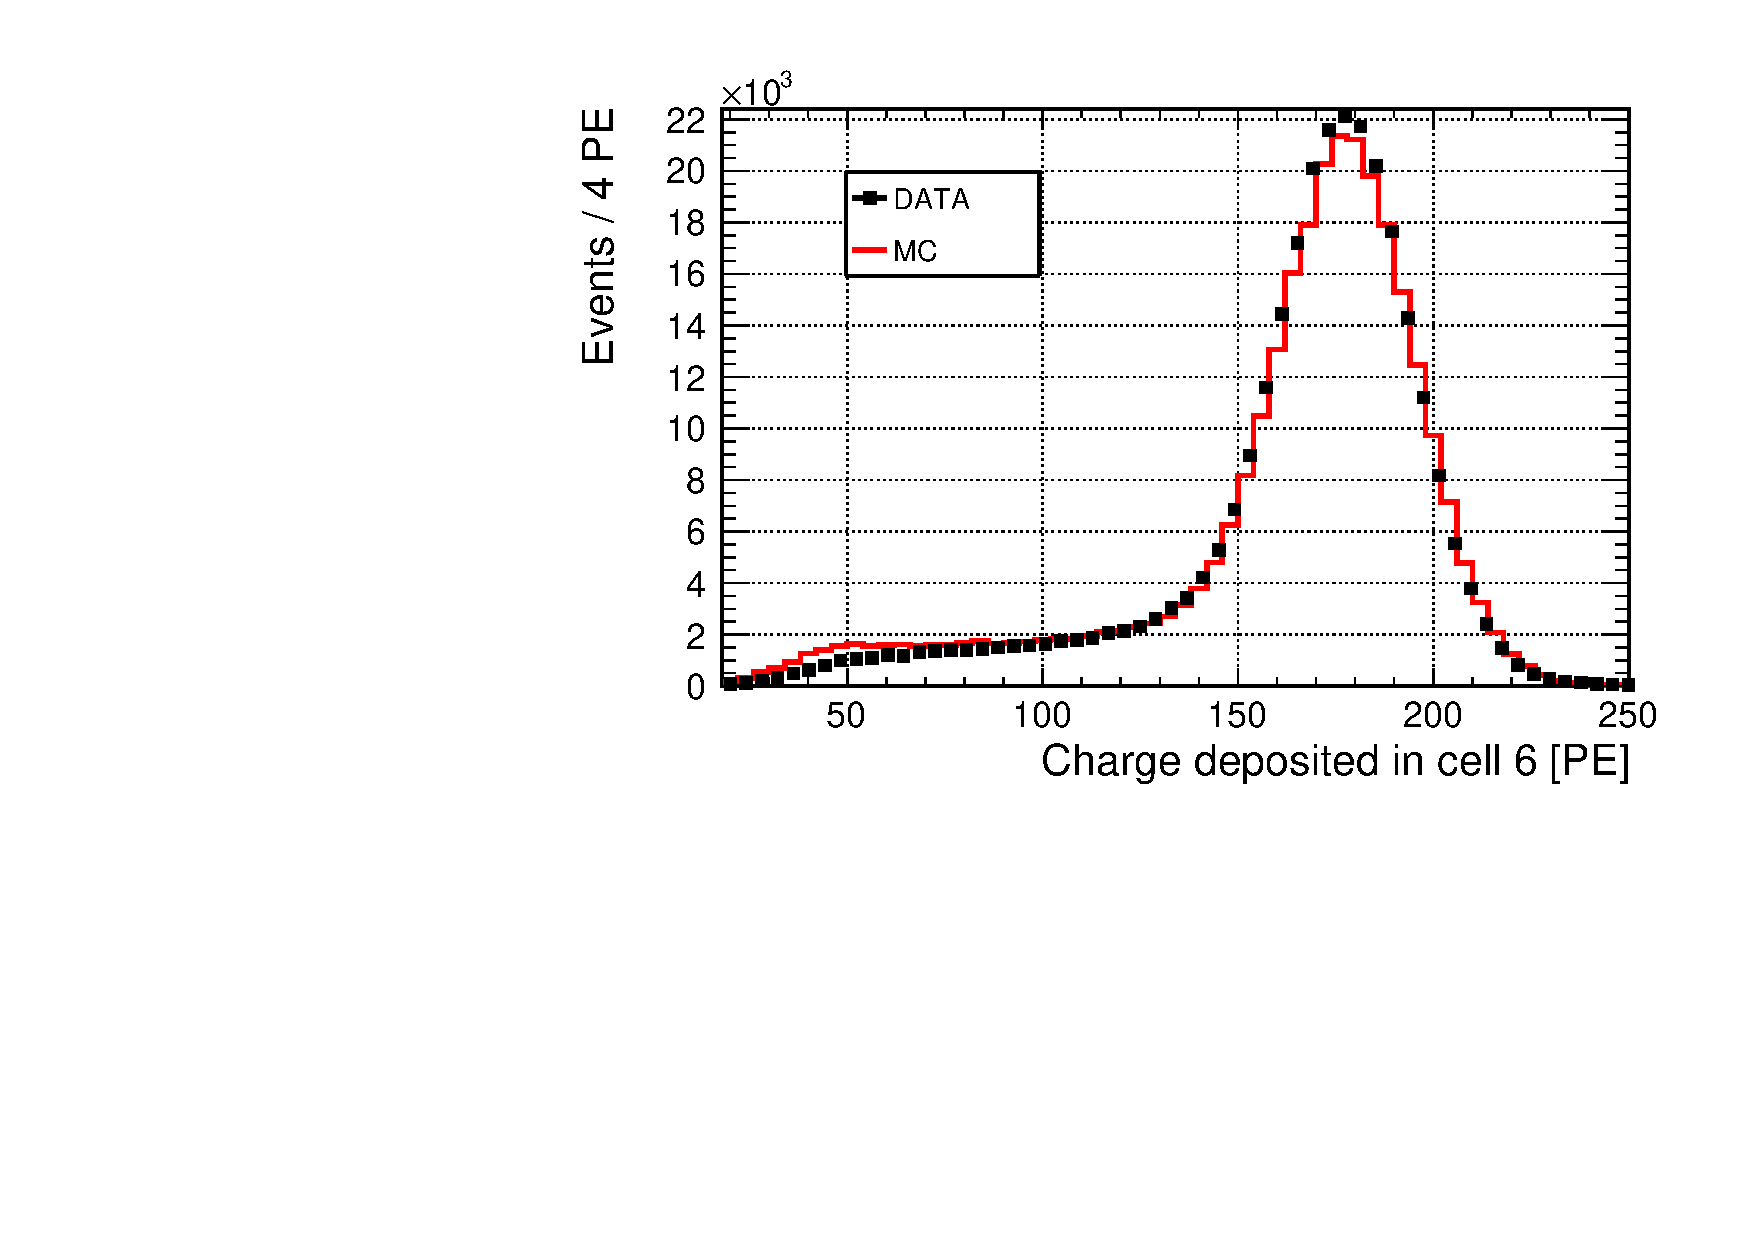
\includegraphics[width=1\textwidth]{images/DataToMCCell6_phase1.pdf}
\caption{}
\label{fig:DataToMCCell6_phase1}
\end{subfigure}
~ % attention ! space sensitive
\begin{subfigure}[b]{0.49\textwidth}
\centering
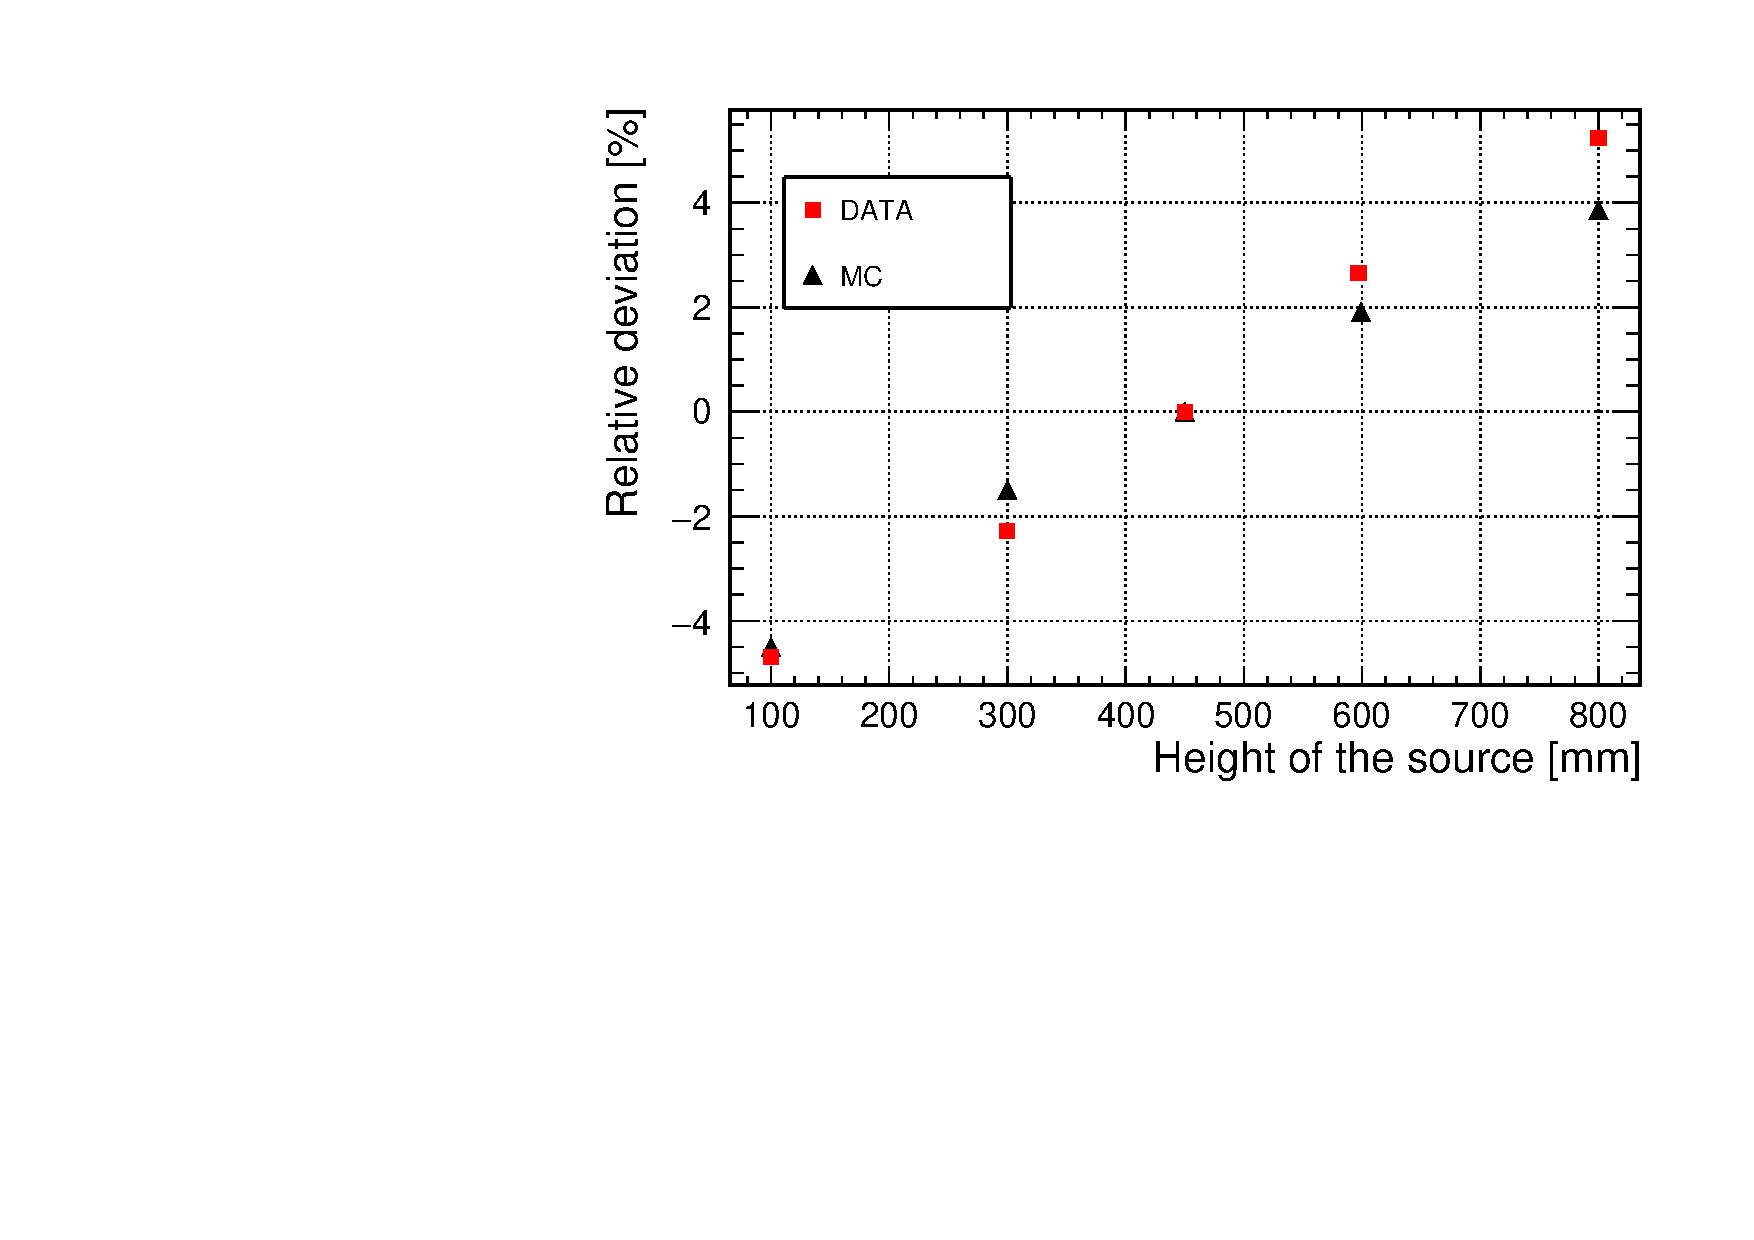
\includegraphics[width=1\textwidth]{images/FivePositionsComparison_cell6.pdf}
\caption{}
\label{fig:FivePositionsComparison_cell6}
\end{subfigure}

\caption[Comparaison des runs ${}^{54}\textrm{Mn}$ entre les données et la simulation]{Comparaison des runs ${}^{54}\textrm{Mn}$ dans les données (noir) et la simulation (rouge). (a) représente le spectre en charge dans la cellule 6 lorsque la source est déployée à mi-hauteur de la cellule. (b) montre les déviations relatives du pic en charge suivant la hauteur de la source par rapport au cas où la source est au centre (450 mm). (source \cite{Allemandou:2018vwb})}
\label{fig:MC_tuning_optics}
\end{figure}

}

\bigbreak

%\begin{itemize}
%    \item Fine tuning data (LL, LY)
%    \item comparaison data
%    \item effets haut bas
%\end{itemize}



\section{Simulation de la cascade gamma Gadolinium}
\label{sec:cascade_Gd_MC}

Avec une concentration de Gadolinium de 0,2 \% de la masse du liquide scintillateur, le temps de capture des neutrons thermiques est réduit à $\SI{16}{\mu s}$, soit un ordre de grandeur de moins qu'avec un liquide scintillateur non dopé où le noyau absorbant principal est l'hydrogène. La capture sur Gadolinium (n-Gd) compte pour 80 \% des captures neutron possibles avec un tel dopage. Le noyau de Gadolinium résultant de l'absorption neutronique se retrouve dans un état excité et finit par décroître sur son état fondamental en émettant plusieurs gammas, dont la somme fait environ $\SI{8}{MeV}$. À cause de la multiplicité des gammas et des longueurs d'interaction typiques de $\SI{20}{cm}$, une large fraction des événements n-Gd est soumise à des fuites d'énergie hors du volume actif. En effet, une mauvaise description du spectre d'émission n-Gd entraine nécessairement une augmentation des incertitudes systématiques sur l'efficacité de détection et donc une augmentation de l'incertitude sur la mesure du flux d'antineutrinos. Malheureusement, les cascades des deux isotopes présents dans le liquide ($\ce{^{156}Gd^*}$ et $\ce{^{158}Gd^*}$) n'ont pas de description expérimentale des schémas de niveaux nucléaires jusqu'à $\SI{8}{MeV}$.\\

Après capture d'un neutron thermique, les noyaux $\ce{^{156}Gd}^*$ et $\ce{^{158}Gd^*}$ ont une énergie d'excitation de $\SI{8.536}{MeV}$ et $\SI{7.937}{MeV}$ respectivement. À ces énergies, la distribution des états excités est considérée comme un continuum dont la densité n'est pas connue expérimentalement. En descendant en énergie, la densité diminue jusqu'à ce que chaque état devienne discernable. Seuls les quelques derniers niveaux d'excitation ont été mesurés expérimentalement, pour le reste de la distribution des niveaux d'énergie une description théorique doit être utilisée.

\bigbreak

%\subsection{Efficacité de détection des neutrons}
%
%\begin{itemize}
%    \item Calcul efficacité avec eff. delta t / eff. coupures / Gd fraction
%    \item Mesures concentration Gd ?
%\end{itemize}


\subsection{Cascade $\gamma$ avec GLG4Sim}

La bibliothèque GLG4Sim est un héritage du code de simulation de Double Chooz \cite{glg4sim_doc}. Celle-ci gère la cascade gamma des deux principaux isotopes ($\ce{^{155}Gd}$ et $\ce{^{157}Gd}$) au sein d'une classe sur mesure connectée à \textsc{Geant4}: \texttt{GdNeutronHPCapture}. La désexcitation des noyaux est traitée soit par des doublets de raies gamma mesurés expérimentalement, soit par la génération d'une cascade suivant une densité d'états théorique. Les doubles raies sont générées à partir des schémas de niveaux mesurés en 1958 par Groshev et al. \cite{Groshev1958}, mais ne comptent que pour 5 \% des cascades tout au plus. Sinon, les cascades sont tirées à partir d'un schéma de niveaux composé de deux états discrets (le fondamental $E_0 \doteq 0$ et le premier niveau excité $E_1$) et un continuum d'états partant de l'énergie $2\times E_1$. La densité d'états pour la transition $E_i \rightarrow E_f$ dans le continuum est donnée par l'expression :

\begin{equation}
    \rho (E_i - E_f) \propto e^{a \sqrt{(E_i - 2E_1) - (E_i - E_f)}},
\end{equation}

\bigbreak

Finalement, la probabilité de faire la transition $E_i \rightarrow E_f$ est proportionnelle à $(E_i - E_f)^3$. Ainsi dans le code, une transition est sélectionnée aléatoirement parmi ces trois cas de figure:\\


% où $\varepsilon$ est l'énergie de la transition. La probabilité qu'un noyau fasse une transition entre deux états est proportionnelle à $\varepsilon^3$. Donc en partant d'un état initial $\varepsilon_i$, trois cas de figure se présentent:\\

\begin{itemize}[label=\textbullet]
    \item Une transition directe sur l'état fondamental : $\Gamma \propto (E_i)^3$,
    \item Une transition sur le premier état excité : $\Gamma \propto (E_i - E_1)^3$, toujours suivie d'une seconde transition vers l'état fondamental $E_1 \rightarrow E_0$,
    \item Une transition dans le continuum : $\Gamma \propto (E_i - E_f)^3 \rho (E_i - E_f) dE_f$.
\end{itemize}

\bigbreak

La procédure est répétée jusqu'à ce que l'état du noyau soit de nouveau sur l'état fondamental. Finalement, à chaque capture neutron, cette méthode génère aléatoirement une cascade de gammas qui emportent toute l'énergie d'excitation. Les dépôts d'énergie de ces gammas sont ensuite simulés avec \textsc{Geant4}.\\

\subsection{Cascade $\gamma$ avec FIFRELIN}

Bien que l'énergie totale de chaque cascade soit conservée avec GLG4Sim, les limitations du modèle théorique se font sentir dans les expériences qui utilisent des détecteurs segmentés et/ou compacts. En effet, dans ces configurations, les gammas de haute énergie sont susceptibles de sortir du détecteur et ainsi peupler la queue de distribution Compton des spectres de réponse. Une description fidèle de la multiplicité et de l'énergie des gammas de cascade est donc requise pour contrôler notamment l'efficacité de détection. L'expérience DANSS, par exemple, a reporté des tensions significatives entre les données de calibration et la simulation dans la partie basse énergie du spectre Gd \cite{Alekseev:2018efk}. De plus, la modélisation précise des cascades Gd est d'une importance capitale pour les détecteurs basés sur le rayonnement Tcherenkov \cite{Hagiwara:2018kmr}. Ici, la production de lumière est très sensible aux énergies des gammas de cascade, car les électrons Compton qu'ils produisent ont une énergie proche de l'énergie seuil Tcherenkov (cf. \ref{seq:scintillation}). Dans \textsc{Stereo}, le léger désaccord entre les données et la simulation sur l'efficacité de détection neutron a aussi été attribué à une mauvaise description de ces gammas de cascade. Cependant, en utilisant les cascades gamma générées à l'aide du code de désexcitation nucléaire \og FIFRELIN \fg{} développé au CEA-Cadarache, les désaccords ont été significativement réduits. Cette étude a fait l'objet d'une publication de la collaboration \textsc{Stereo} \cite{AlmazanMolina:2019aoc}.\\

À l'origine, FIFRELIN est un code de désexcitation nucléaire qui a été développé pour prédire les propriétés des neutrons et gammas issus de fragments de fission. Le code est divisé en deux parties: attribution des états initiaux à partir d'un fragment de fission, et la modélisation du processus de désexcitation nucléaire. Les états initiaux du $\ce{^{156}Gd}^*$ et du $\ce{^{158}Gd^*}$ étant déjà connus, \textsc{Stereo} ne se sert que de la deuxième partie du code. Une fois que l'état initial est spécifié, FIFRELIN est capable de générer une multitude de cascades tout en prenant en compte les incertitudes théoriques sur la structure nucléaire. Pour cela, le code utilise toute la connaissance expérimentale des schémas de niveaux, et l'information manquante est traitée par les modèles nucléaires. Finalement, les cascades sont générées suivant trois méthodes d'échantillonnages différentes suivant la plage en énergie:\\

\afterpage{

\begin{figure}[h!]

\centering
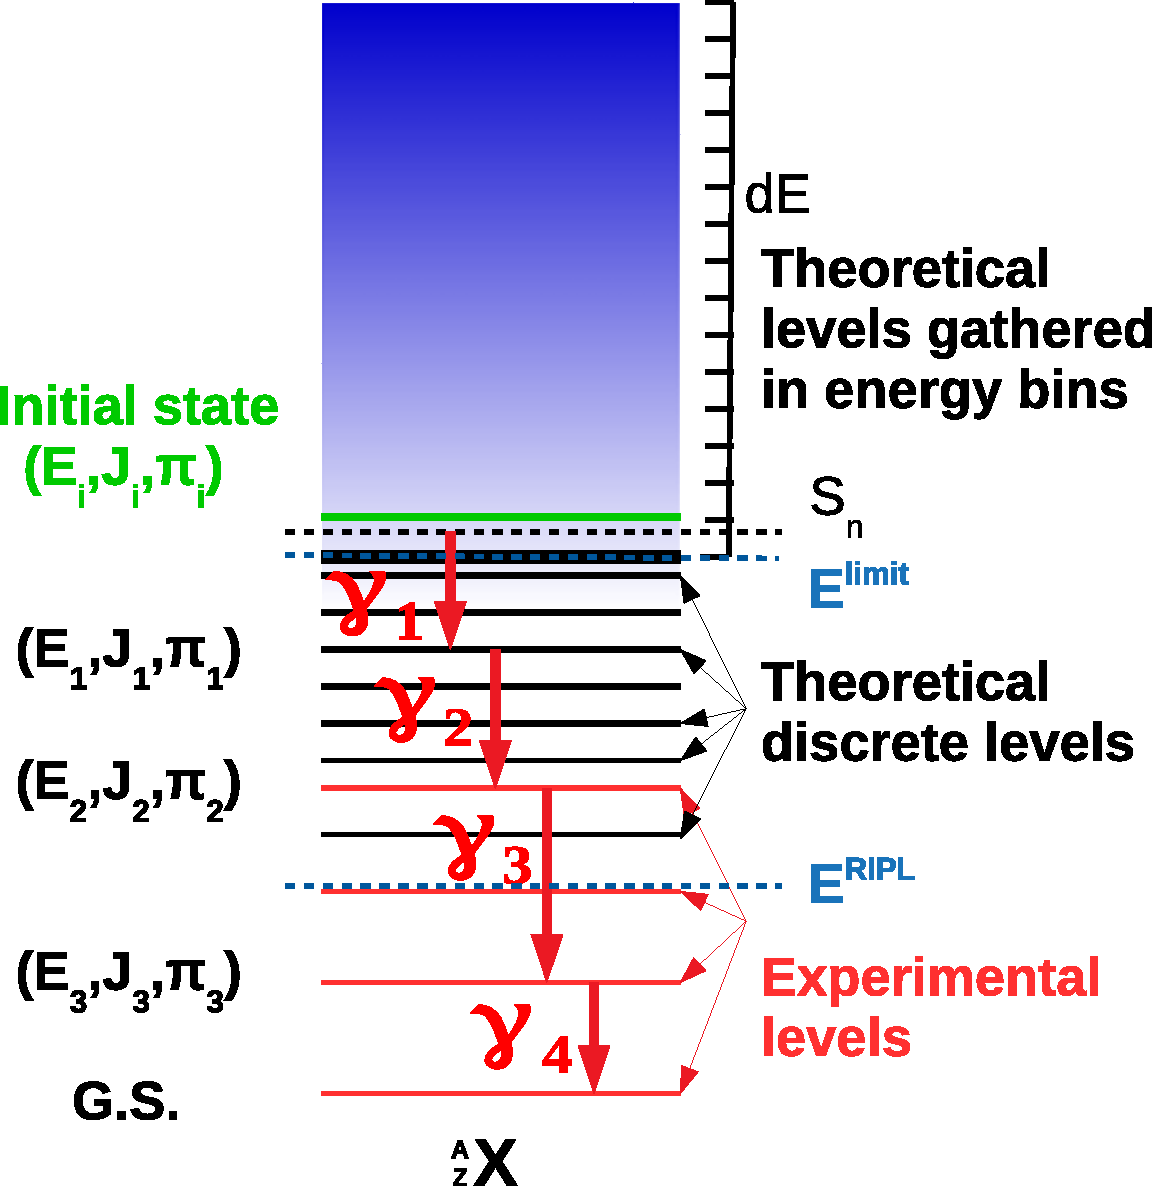
\includegraphics[width=0.49\textwidth]{images/FIFRELIN_model.pdf}
\caption[Schéma représentant une cascade gamma générée par FIFRELIN]{Schéma représentant une cascade gamma générée par FIFRELIN. La ligne verte correspond à l'état initial du noyau de Gd qui vient de capturer un neutron.}
\label{fig:FIFRELIN_model.pdf}

\end{figure}

}

\begin{itemize}[label=\textbullet]
    \item Lorsque $E > E^\textrm{limit}$, les niveaux d'excitation sont indénombrables et donc répartis sur un continuum dont la densité d'états est conduite par un modèle théorique: $\rho(E,J, \pi)$. En pratique, les niveaux sont rassemblés en bin en énergie $E$ à spin-parité fixé par le modèle ($J^\pi$).\\
    \item Lorsque $ E^\textrm{RIPL} < E \leq E^\textrm{limit}$, les niveaux sont dénombrables, mais peu ont été déterminées par l'expérience. Les niveaux d'excitation additionnels sont échantillonnés jusqu'à ce que la densité de niveaux prédite $\rho(E,J, \pi)$ soit satisfaite.\\
    \item Pour $E \leq E^\textrm{RIPL}$, tous les niveaux d'excitation sont expérimentalement connus et récupérés dans la base de données nucléaire RIPL-3 \cite{Capote:2009qqf}. Si des états de spin ou de parité sont manquants, FIFRELIN les échantillonne à partir du modèle théorique.\\
\end{itemize}

Ces trois régimes sont présentés sur la figure \ref{fig:FIFRELIN_model.pdf}. Par rapport à GLG4Sim, FIFRELIN utilise une description plus complète de la densité de niveau. Cette dernière prend en compte à la fois l'énergie $E$, l'état de spin $J$ et la parité $\pi$ :

\begin{equation}
    \rho(E, J, \pi) = \rho_\textrm{tot}(E) \times P(J|E) \times P(\pi),
\end{equation}

\bigbreak

où $\rho_\textrm{tot}(E)$ est la densité de niveaux nucléaires totale (sans se soucier du couple spin-parité $J^\pi$), $P(J|E)$  la distribution du moment cinétique en fonction de l'énergie et $P(\pi)$ la probabilité d'avoir une parité $\pm 1$. Les deux états de parité sont supposés équiprobables, c'est-à-dire $P(\pi = \pm 1) = 0.5$. Les états de la structure hyperfine sont paramétrisés par une gaussienne de largeur $\sigma(E)$ qui exprime la dispersion du moment angulaire nucléaire \cite{Bethe:1936zza}:

\begin{equation}
    P(J|E) = \frac{2J + 1}{2 \sigma^2(E)} \textrm{exp}\left(- \frac{(J + 1/2)^2}{2 \sigma^2(E)}\right).
\end{equation}

\bigbreak

Finalement, la densité de niveaux $\rho_\textrm{tot}(E)$ est donnée par le \og Composite Gilbert Cameron Model \fg{} (CGCM) \cite{doi:10.1139/p65-139}, qui est la combinaison d'une fonction de densité de niveaux selon un modèle à température nucléaire constante pour la partie basse énergie et un modèle de gaz de Fermi à haute énergie.\\

\afterpage{

\begin{figure}[h!]

\centering
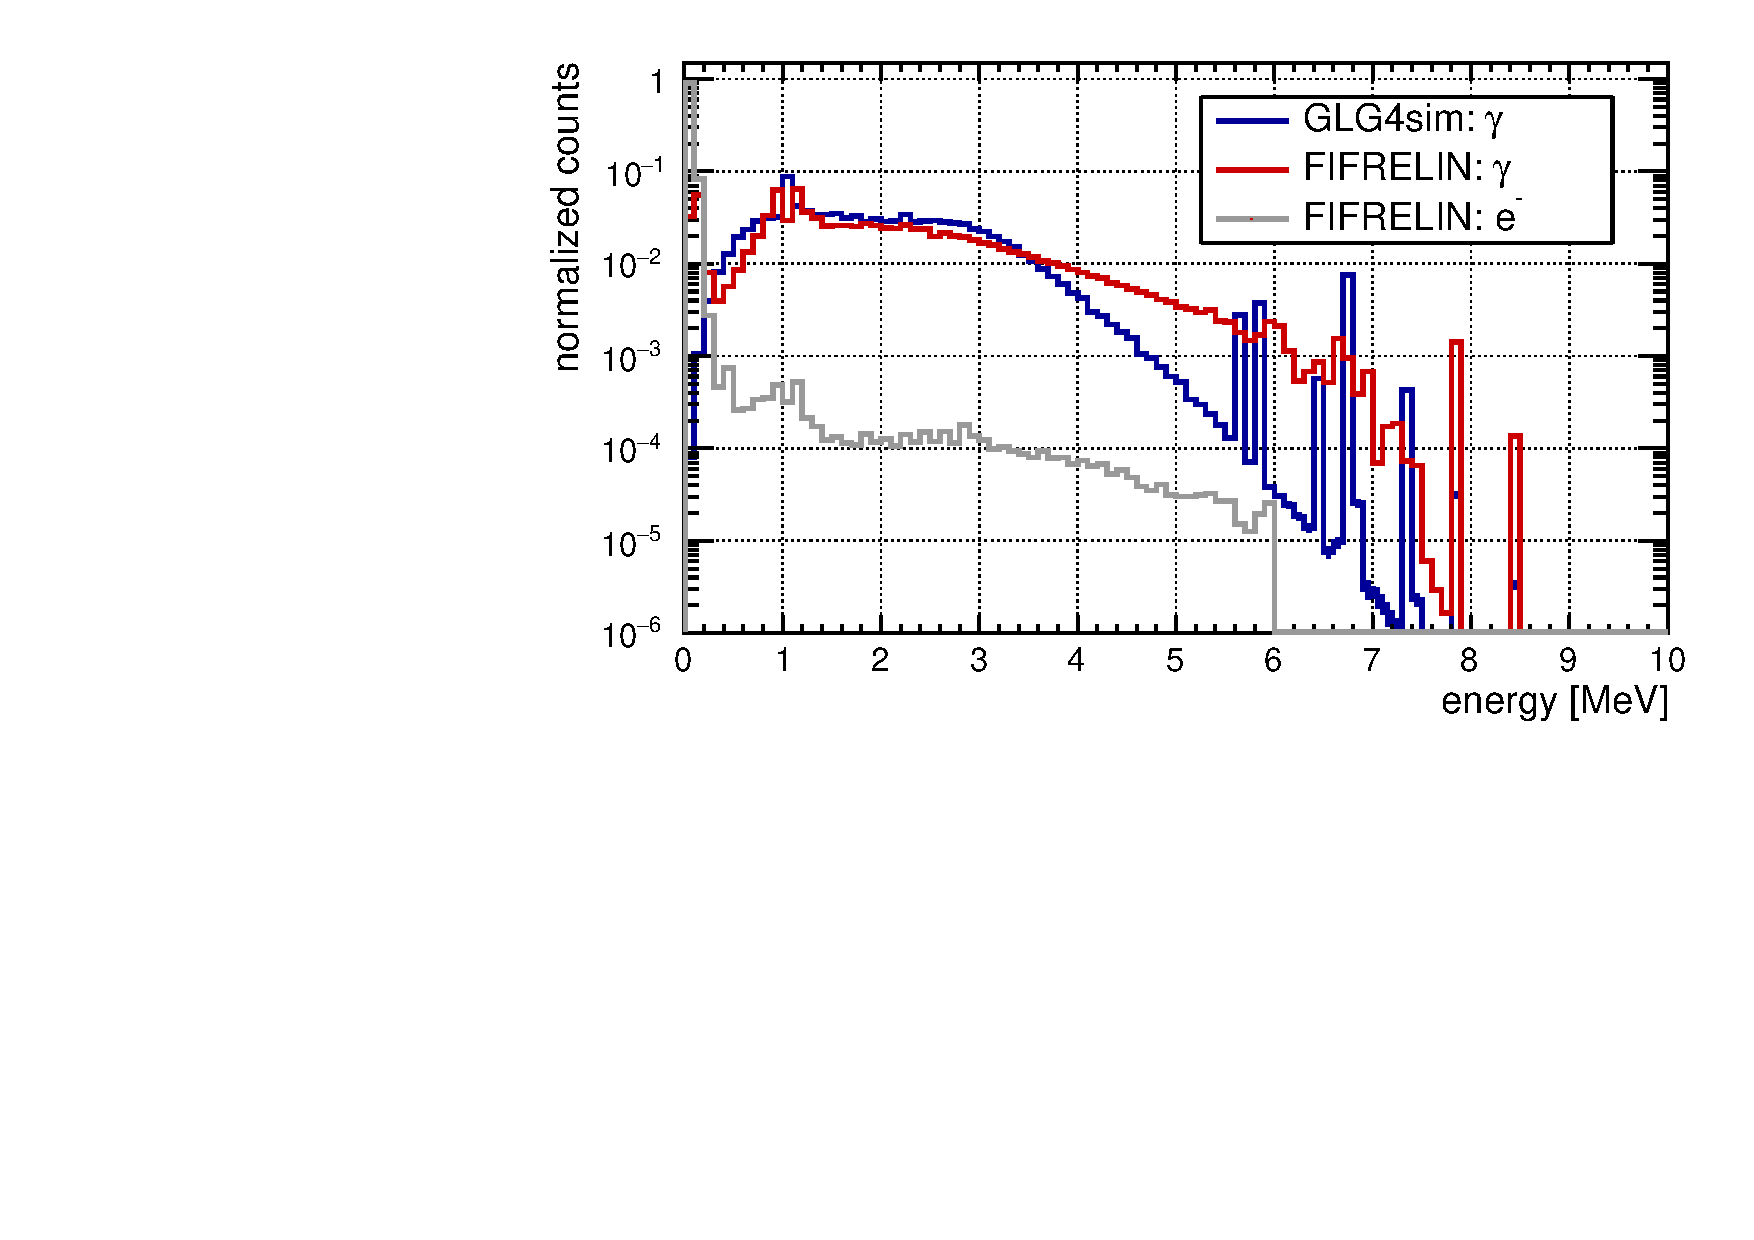
\includegraphics[width=0.8\textwidth]{images/FIFRELIN_vs_GLG4Sim.pdf}
\caption[Spectres en énergie des produits de désexcitation du Gadolinium]{Spectres en énergie des produits de désexcitation du Gadolinium. La simulation GLG4Sim ne génère que des gammas (bleu), alors que FIFRELIN fourni à la fois des gammas (rouge) et des électrons de conversion (gris).}
\label{fig:FIFRELIN_vs_GLG4Sim.pdf}

\end{figure}

}

Au moment d'une désexcitation, FIFRELIN calcule toutes les transitions possibles $\Gamma_p(i \rightarrow f)$ depuis un état initial $i$ vers un état final $f$ avec émission d'une particule $p$, puis parmi ces transitions une seule est échantillonnée. La procédure est répétée jusqu'à ce que le noyau soit retombé sur l'état fondamental. Ainsi pour chaque cascade tirée, FIFRELIN fourni une série d'électrons de conversion et de gammas avec leurs propriétés: énergie, multipolarité, et mode (E ou B). La comparaison des spectres de particules émises avec FIFRELIN et GLG4Sim présentée sur la figure \ref{fig:FIFRELIN_vs_GLG4Sim.pdf}, montre des différences significatives dans la distribution en énergie des gammas des cascades de désexcitation.\\

Finalement, la comparaison des simulations FIFRELIN et GLG4Sim avec les véritables données \textsc{Stereo} est décrite dans la section \ref{sec:neutrino_biases_eff}.

\bigbreak

\section{Simulation des bruits de fond cosmiques}

Les bruits de fond d'origine cosmique sont définis comme étant des particules qui atteignent le détecteur alors qu'elles ont été créées dans l'atmosphère par une chaine de réactions déclenchée à l'origine par un rayon cosmique. Bien qu'ils constituent la source de bruit de fond principale au signal neutrino, ils permettent aussi de tester la réponse en énergie du détecteur indépendamment du dispositif de calibration. La simulation de ces bruits de fond est donc cruciale pour estimer les incertitudes systématiques et contraindre les distorsions de l'échelle en énergie.\\

\afterpage{

\begin{figure}[h!]
\centering
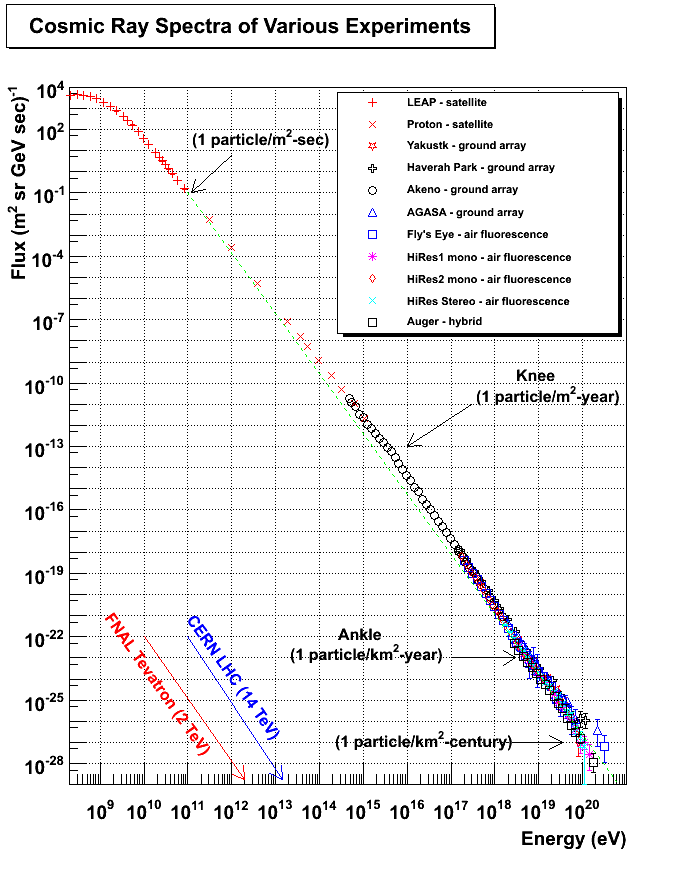
\includegraphics[width=0.59\textwidth]{images/CR_spec.png}
\caption[Spectre du flux de rayons cosmiques mesuré par de multiples expériences]{Spectre du flux de rayons cosmiques mesuré par de multiples expériences. (source \cite{whanlon})}
\label{fig:CR_spec.png}


\end{figure}

\begin{figure}[h!]
\centering
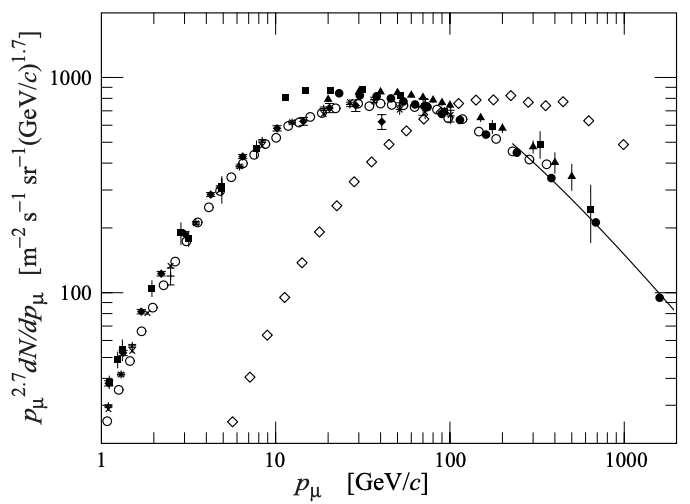
\includegraphics[width=0.65\textwidth]{images/muon_spectrum.png}
\caption[Spectres des muons cosmogéniques mesurés au niveau de la mer]{Spectres des muons cosmogéniques mesurés au niveau de la mer. Les losanges représentent le spectre des muons qui ont un angle d'incidence $\theta = 75^{\circ}$, tandis que les autres points sont différentes mesures pour $\theta = 0^{\circ}$ (incidence normale). L'exposant $2.7$ sur l'axe vertical est utilisé pour comparer l'allure du spectre avec celui des rayons cosmiques qui décroit en $E^{-\gamma -1}$ en dessous de $10^{15} \SI{}{eV}$ (cf Eq. (\ref{eq:cosmic_power_law})). (source : \cite{PDG_particle_matter_2018})}
\label{fig:muon_spectrum.png}


\end{figure}

\clearpage

}

Les rayons cosmiques sont des particules relativistes qui atteignent l'atmosphère terrestre et dont le spectre en énergie s'étale jusqu'à $10^{20}\SI{}{eV}$ (limite de Greisen-Zatsépine-Kouzmine) \cite{Greisen:1966jv}. Leur origine et leur mécanisme de production restent encore en discussion aujourd'hui, surtout à très haute énergie. Le spectre en énergie des rayons cosmiques a été mesuré avec divers instruments depuis la centaine de $\SI{}{MeV}$ et est présenté sur la figure \ref{fig:CR_spec.png}. Un modèle composé de plusieurs lois de puissance décrit l'ensemble du spectre en énergie :

\begin{equation}
\label{eq:cosmic_power_law}
    \frac{dN}{dE} \propto E^{-\gamma - 1},
\end{equation}

\bigbreak

où $\gamma = 1.7$ entre $10^8$ et $10^{15}\SI{}{eV}$, $\gamma = 2$ entre $10^{15}$ et $10^{19}\SI{}{eV}$, et finalement $\gamma = 2.3$ au-dessus. La transition entre la première et seconde phase du spectre est appelé le genou (\textit{knee}), et celle entre la seconde et la troisième phase est appelé cheville (\textit{ankle}). En dessous de $10^{10}\SI{}{eV}$, les particules sont principalement d'origine solaire, tandis que jusqu'à $10^{15}\SI{}{eV}$, elles sont d'origine galactique. Le reste des particules cosmiques sont d'origine extragalactique. Les particules cosmiques qui induisent le plus de bruits de fond dans \textsc{Stereo} sont d'origine solaire, et leur flux est soumis aux cycles solaires ($\simeq 11$ ans). La soustraction du bruit de fond pour extraire le signal neutrino est effectuée en comparant les périodes où le réacteur est ON avec celles où le réacteur est OFF: le bruit de fond doit être comparable entre les deux périodes. C'est pourquoi la compréhension des variations du bruit induit par les cosmiques est cruciale pour l'analyse de \textsc{Stereo}. Les principaux paramètres sont discutés dans la suite de cette section et le contrôle fin de ces variations pour l'extraction des taux de neutrinos est discuté au Chapitre \ref{chap:chapitre_analysie}.\\

% Dis plutôt que les variations du bruit induit par les cosmiques sont cruciales pour l'analyse de STEREO, que les principaux paramètres sont discutés dans la suite de cette section et que le contrôle fin de ces variations pour l'extraction des taux de neutrinos est discuté au chapitre XX.

Les rayons cosmiques sont composés de particules neutres, comme les photons et les neutrinos, mais aussi de particules chargées: principalement des noyaux (99\%), contre 1\% d'électrons libres. Parmi ces noyaux, 90\% sont des protons et 9\% sont des particules alpha. Le reste se compose de noyaux plus lourds. Ces particules sont appelées particules \og \textit{primaires} \fg{}. Ces particules entrent en collision avec les noyaux composant l'atmosphère --- principalement avec l'azote 14 et l'oxygène 16 --- et entrainent la création de particules dites \og \textit{secondaires} \fg{} telles que des pions ou des kaons. Ces mésons, qui ont une durée de vie très courte ($< 10^{-8}\SI{}{s}$), se désintègrent dans l'atmosphère majoritairement par ces canaux:

\begin{align}
    \ce{\pi^{\pm} \rightarrow \mu^{\pm} + \nu_{\mu}}\\
    \ce{K^{\pm} \rightarrow \mu^{\pm} + \nu_{\mu}}.
\end{align}

\bigbreak

Les muons produits ont des impulsions allant jusqu'au TeV et sont donc qualifiés de relativistes. Cela leur procure la possibilité de descendre jusqu'au niveau de la mer (environ $\SI{15}{km}$) malgré leur courte durée de vie. Pour les moins énergétiques d'entre eux, la désintégration en électron se produit et la composante du flux muon à basse énergie est tuée. Le spectre en énergie des muons mesuré au niveau de la mer est présenté sur la figure \ref{fig:muon_spectrum.png}.

\bigbreak

Le flux de particules d'origine cosmique qui est susceptible d'atteindre \textsc{Stereo} dépend de la quantité d'atmosphère qu'elles doivent traverser. Ce flux est représenté en fonction du grammage atmosphérique sur la figure \ref{fig:cosmic_vs_grammage.png}. Au niveau du sol, le flux est composé très majoritairement de muons ($\pm$): ce sont eux qui engendrent le plus de bruits de fond dans le détecteur. De plus, puisque la quantité de muons incidents dépend du grammage de l'atmosphère, le flux muonique est anti-corrélé avec la pression atmosphérique.\\


\afterpage{

\begin{figure}[h!]
\centering
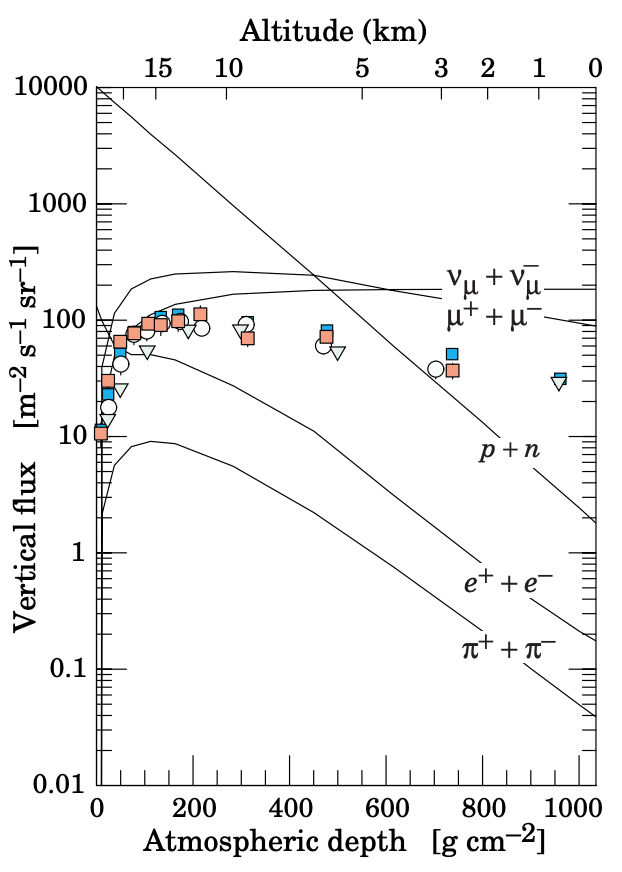
\includegraphics[width=0.46\textwidth]{images/cosmic_vs_grammage.png}
\caption[Flux de particules d'origine cosmiques en fonction du grammage atmosphérique]{Flux de particules d'origine cosmiques en fonction du grammage atmosphérique. Au niveau de la mer, les composantes dominantes sont celle des neutrinos et des muons ($\pm$). (source : \cite{PDG_particle_matter_2018})}
\label{fig:cosmic_vs_grammage.png}

\end{figure}

\begin{figure}[h!]
  \centering
  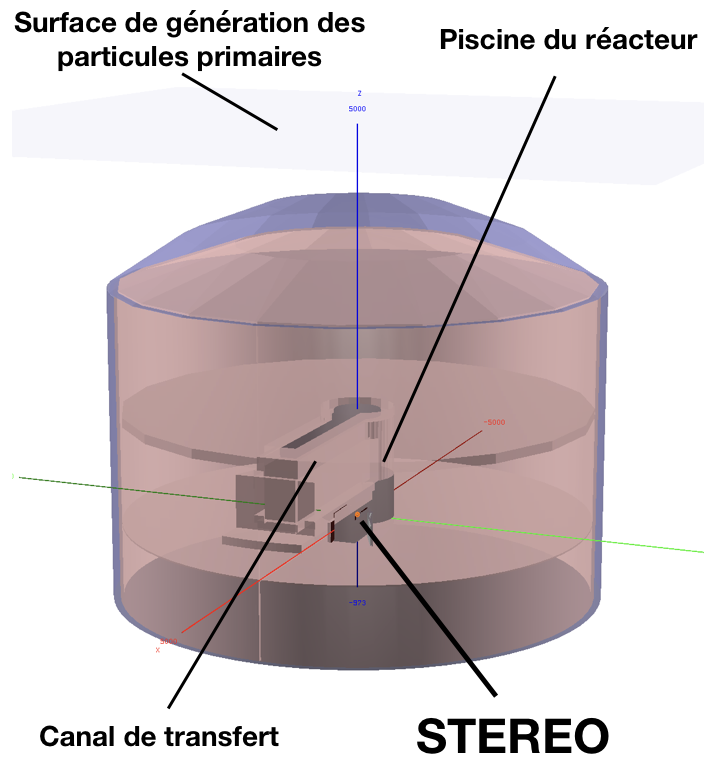
\includegraphics[width=0.55\linewidth]{images/CRY_figure.png}
  \caption[Géométrie du hall expérimental de l'ILL implémenté dans les simulations CRY]{Géométrie du hall expérimental de l'ILL implémenté dans les simulations CRY. La casemate de \textsc{Stereo} se situe sous le canal de transfert qui lui offre un blindage supplémentaire contre les bruits de fond d'origine cosmique. (source : \cite{docdb354})}
  \label{fig:CRY_figure}
\end{figure}


\clearpage

}

Une modélisation rigoureuse de ces bruits de fond d'origine cosmique est cruciale. C'est l'objet de la partie suivante.

\bigbreak

%\begin{itemize}
%    \item Production des muons cosmiques
%    \item Distribution en énergie
%    \item Dépendance avec la pression atm ? (grammage atm vs rayons cosmiques)
%\end{itemize}

\subsection{Simulation des gerbes cosmiques}

Le code de simulation \textit{CRY} \cite{CRY} a été exploité pour simuler la génération des bruits de fond cosmiques dans l'atmosphère ainsi que leur temps d'arrivée et leur angle zénithal. La bibliothèque \textit{CRY} génère des gerbes de particules corrélées à plusieurs altitudes: $\SI{11300}{m}$, $\SI{2100}{m}$ et au niveau de la mer. Pour \textsc{Stereo}, les simulations au niveau de la mer sont utilisées avec un facteur d'amplification de $\SI{1.279}{}$ pour tenir compte de l'altitude du site ($\SI{210}{m}$). Les particules primaires sont générées sur une surface de $\SI{300}{m^2}$, à $\SI{50}{m}$ au-dessus du détecteur. Pour tenir compte de l'atténuation du flux cosmique en fonction de l'angle d'arrivée des particules, la géométrie du hall de l'ILL est implémentée tout comme le canal de transfert et la piscine du réacteur (voir figure \ref{fig:CRY_figure}). La propagation des particules générées par \textit{CRY} est ensuite simulée avec le code de simulation \textsc{Geant4} \cite{docdb354}. Pour des raisons d'optimisation du temps de calcul, seules les particules primaires dont la direction pointe vers le centre du détecteur à $\pm \SI{10}{m}$ sont simulées.

\bigbreak


La plupart des particules qui atteignent et produisent un signal dans le détecteur sont des muons. En effet en plus d'être la particule cosmique la plus abondante au niveau de la mer, leur fort pouvoir pénétrant leur procure la possibilité de traverser à la fois le canal d'eau et les blindages \textsc{Stereo}. Des mesures dédiées à la dépendance angulaire du flux muonique ont été confrontées aux simulations CRY \cite{zsoldos:tel-01575951} et ont montré la haute fidélité du processus de simulation (voir figure \ref{fig:muon_flux_PN3.png}). Le taux de comptage simulé s'est montré en accord avec les données mesurées à $\pm \SI{10}{\%}$ près \cite{docdb354}.\\

% De plus, la forme des spectres en charge est bien reproduite dans la simulation jusque $\SI{60}{MeV}$, ce qui contraint les effets de non-linéarité sur la mesure du nombre de photo-électrons.\\

\afterpage{

\begin{figure}[h!]
\centering
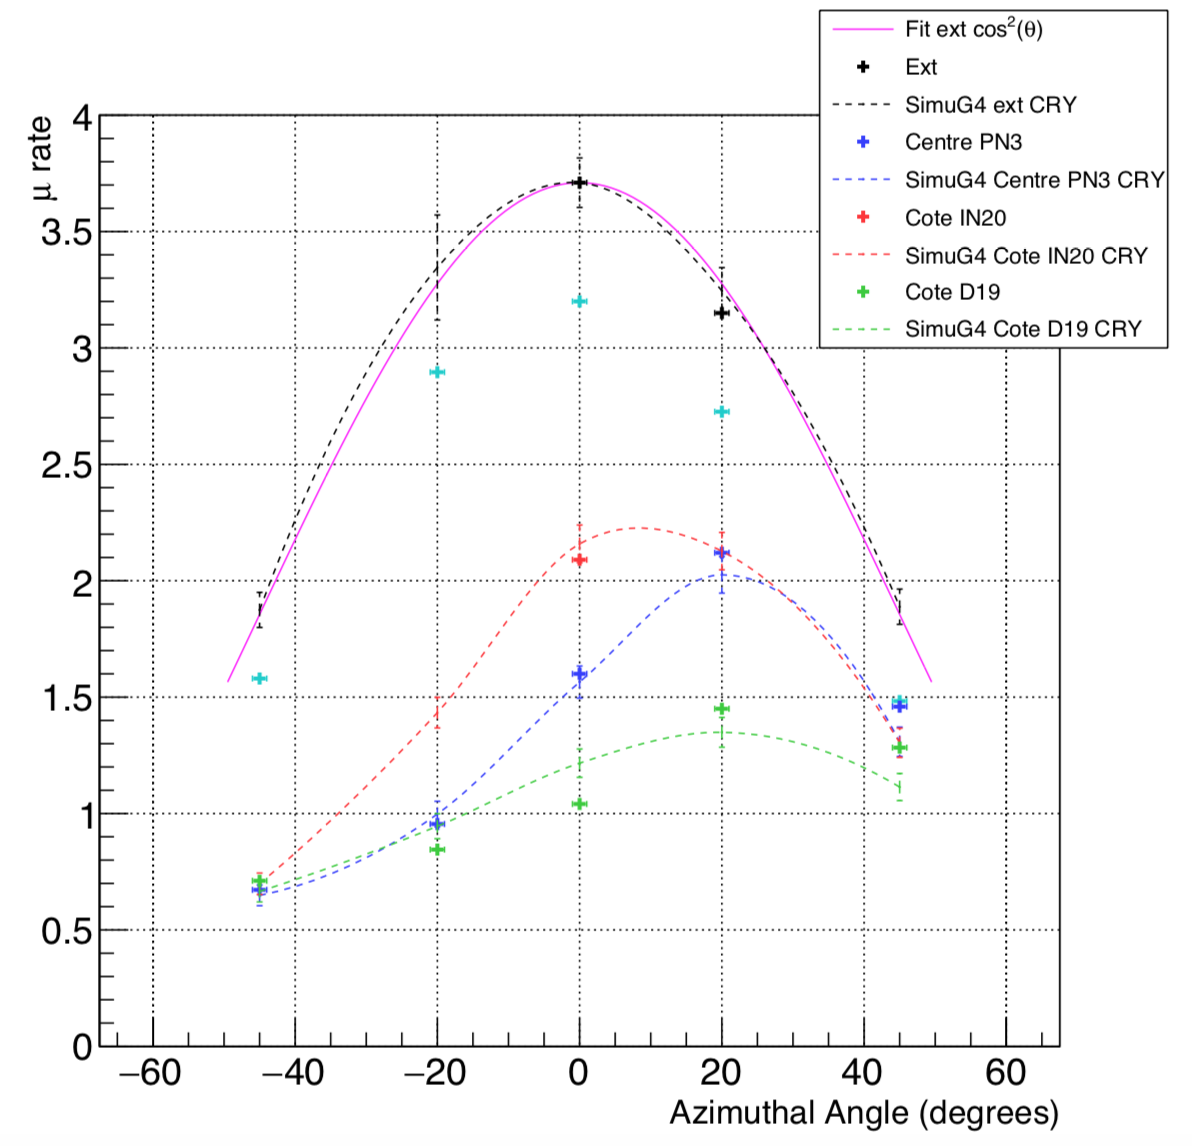
\includegraphics[width=0.65\textwidth]{images/muon_flux_PN3.png}
\caption[Comparaison de la dépendance angulaire des muons entre les données et la simulation]{Comparaison de la dépendance angulaire des muons entre les données et la simulation. Les points représentent les mesures réalisées avec une roue cosmique à différents emplacements et les courbes en pointillé sont le résultat des simulations CRY. Les éléments en noir correspondent à la dépendance angulaire du flux de muons à l'extérieur du bâtiment de l'ILL tandis que les couleurs rouges, vertes, et bleues sont respectivement des mesures réalisées dans la casemate \textsc{Stereo} du côté IN20, D19 et au centre. L'importante suppression des angles azimutaux négatifs dans la casemate est essentiellement due à la présence du canal de transfert au-dessus. (source : \cite{zsoldos:tel-01575951})}
\label{fig:muon_flux_PN3.png}


\end{figure}

}

% Figure 4.33 Stephane

\bigbreak


Les simulations de muons cosmogéniques sont exploitées à plusieurs fins. Tout d'abord, elles permettent d'identifier les coupures topologiques à employer pour isoler les signaux neutrinos. Ces études sont décrites dans la section \ref{sec:energy_cuts}. Ensuite, lorsque les muons traversent des matériaux, ils peuvent induire la création de neutrons en interagissant avec les noyaux par spallation. Les neutrons qui atteignent le volume cible du détecteur peuvent être capturés par les noyaux de Gadolinium et d'hydrogène. Les gammas de désexcitation de ces noyaux sont détectés et permettent de tester les effets de volume sur l'échelle en énergie. La simulation de ces événements est décrite dans la section suivante.

\bigbreak

%\begin{itemize}
%    \item Production des particules dans l'atmosphère
%    \item Spectre en E des muons
%    \item Distribution angulaire
%    \item Simulations CRY
%\end{itemize}

\subsection{Les gammas issus des captures neutron}
\label{sec:sim_gamma_from_nX}

La plupart des neutrons issus de la spallation d'un muon sur un noyau sont créés dans les matériaux dont les constituants sont lourds : $\ce{^{A}_{Z}X}$, où A est élevé \cite{Formaggio:2013kya}. C'est pourquoi la plupart des neutrons cosmogéniques sont créés dans les blindages en plomb, comme le montre la figure \ref{fig:all_neutron_creation_vertices.png}. Certains de ces neutrons sont capturés par un noyau d'hydrogène dans les alentours du détecteur ou directement par le Gadolinium dans le liquide. Les gammas de désexcitation sont finalement détectés s'ils déposent de l'énergie dans le liquide. La répartition des dépôts d'énergie dans le liquide est différente de celle utilisée pour la calibration avec les sources internes. Elle est attendue plus homogène et donc comparable à celle des interactions des neutrinos. Ainsi, les erreurs systématiques sur la réponse en énergie sont déterminées en comparant l'énergie reconstruite de ces gammas entre les données et la simulation. Il est donc crucial de décrire correctement toute la chaîne d'interaction des muons jusqu'à la capture neutron pour obtenir une répartition des dépôts d'énergie réaliste.\\

\afterpage{

\begin{figure}[h!]
\centering
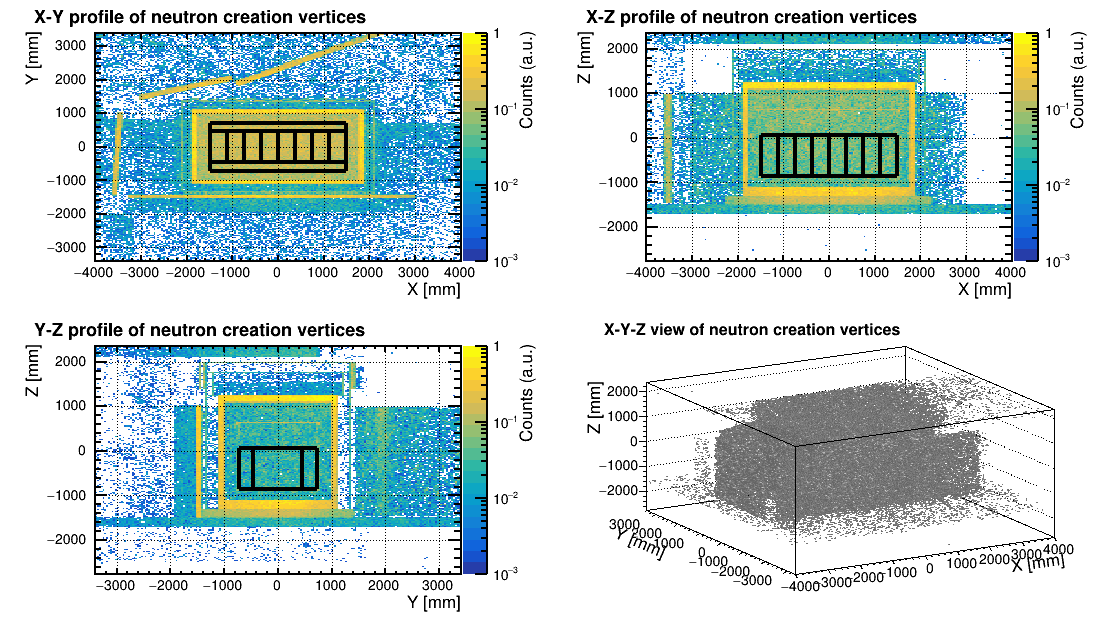
\includegraphics[width=1\textwidth]{images/all_neutron_creation_vertices.png}
\caption[Distribution spatiale des neutrons créés par spallation]{Distribution spatiale des neutrons créés par spallation. Puisque les réactions de spallation sont favorisées sur les matériaux lourds, les blindages en Plomb apparaissent en surbrillance.}
\label{fig:all_neutron_creation_vertices.png}

\end{figure}

}

Afin de sélectionner ce signal dans les données, une recherche de paires corrélées en temps est exploitée, dans laquelle un signal muon est attendu dans la fenêtre Prompt tandis que le signal de la capture neutron est escompté dans la fenêtre Retardée. Les muons qui ont déposé au moins $\SI{3}{MeV}$ sont acceptés dans la fenêtre Prompt, c'est pourquoi seuls les vertex de création de neutrons qui sont associés avec un muon respectant ce critère sont simulés. La majorité des neutrons à l'étude sont créés dans le plomb en dessous du détecteur. Bien que ce point chaud ne soit pas en directe proximité avec le volume actif, l'énergie cinétique des neutrons est suffisante (quelques MeV) pour qu'une fraction passe les blindages et se fassent capturer proche du détecteur.\\

La majorité des captures neutron sur hydrogène se situent dans le blindage intérieur en polyéthylène (lui-même riche en protons) et, dans une moindre mesure, d'autres captures se produisent directement dans le liquide. Cependant pour être détectés, les gammas doivent déposer de l'énergie dans le liquide scintillateur donc la composante des gammas provenant du blindage est drastiquement réduite. En définitive, la majorité des gammas de capture qui passent les coupures en énergie proviennent soit directement du liquide, soit de la plaque de polyéthylène en bas du détecteur (voir figure \ref{fig:neutron_capture_vertices.png}). À $\SI{2.2}{MeV}$, l'interaction dominante des gamma est la diffusion Compton. Le processus de scintillation est déclenché par l'électron fils de cette réaction, donc la position de la première interaction des gammas montre où l'énergie est déposée. La figure \ref{fig:firsthit_gamma_vertices.png} montre que les dépôts d'énergie se rapprochent de la distribution spatiale des neutrinos avec une distribution plate en X, plate en Y, mais avec un excès d'événements en bas qui peut être corrigé \textit{a posteriori} à l'aide des calibrations $\ce{^{54}Mn}$. C'est cette distribution des dépôts d'énergie qui sert à l'estimation des incertitudes systématiques sur l'échelle en énergie (c.f. section \ref{sec:pic_gamma_nH}).\\

\bigbreak

\afterpage{

\begin{figure}[h!]
\centering
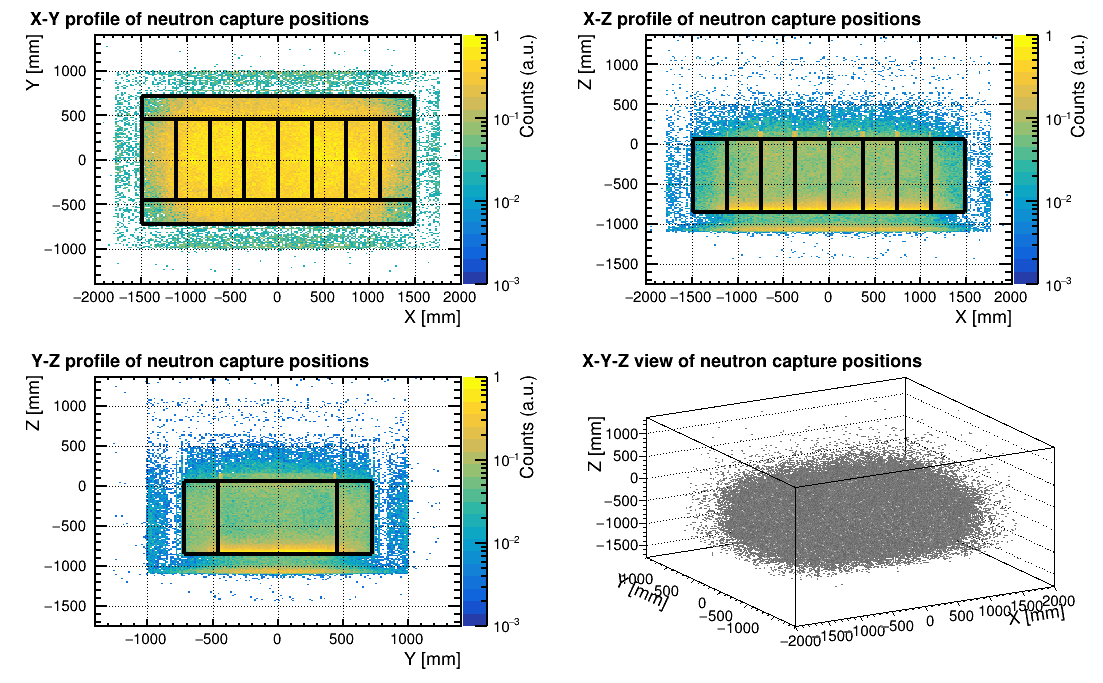
\includegraphics[width=1\textwidth]{images/neutron_capture_vertices.png}
\caption[Distribution spatiale des captures neutrons sur les noyaux d'hydrogène]{Distribution spatiale des captures neutrons sur les noyaux d'hydrogène. Cette fois les points chauds sont majoritairement situés dans les milieux hydrogénés: liquide scintillateur, polyéthylène, ou encore buffers en acrylique. Puisque les noyaux d'hydrogène excités sont émetteurs de la raie gamma à $\SI{2.2}{MeV}$, ces distributions correspondent aussi à la position d'émission des gammas.}
\label{fig:neutron_capture_vertices.png}

\end{figure}
\begin{figure}[h!]
\centering
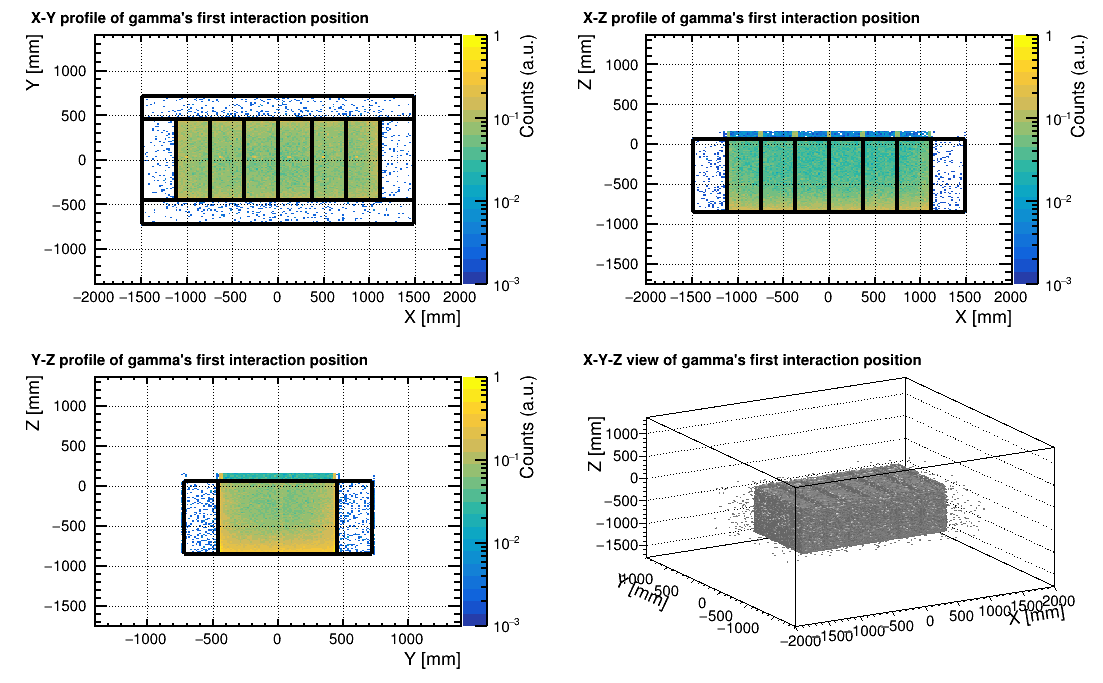
\includegraphics[width=1\textwidth]{images/firsthit_gamma_vertices.png}
\caption[Distribution spatiale des premières interactions gamma dans le détecteur]{Distribution spatiale des premières interactions gamma dans le détecteur. À $\SI{2.2}{MeV}$, le canal d'interaction principal des gamma est la diffusion Compton. Puisqu'une grande fraction de leur énergie est cédée à l'électron dès la première interaction \cite{PhysRev.21.483}, ces distributions indiquent au premier ordre la position des dépôts d'énergie dans le liquide.}
\label{fig:firsthit_gamma_vertices.png}

\end{figure}

\clearpage
}


%\begin{itemize}
%    \item Utilité de ces gammas
%    \item Distribution des vertex neutron / spectres / multiplicité
%    \item Distribution des gammas de capture
%\end{itemize}

\section{Simulation des neutrinos}
\label{sec:neutrino_simulation}

L'intérêt de \textsc{Stereo} réside dans le fait de s'affranchir des prédictions du spectre neutrino émis par le réacteur de l'ILL en comparant les déformations relatives des spectres dans chaque cellule. Si les déformations observées sont compatibles avec un motif d'oscillation, alors la présence d'une nouvelle famille de neutrino peut être affirmée sans ambiguïté, c'est-à-dire sans pouvoir douter de la validité de la prédiction utilisée. C'est la tâche principale à laquelle s'est attelée \textsc{Stereo} jusqu'en 2018. Cependant, \textsc{Stereo} offre aussi la possibilité de mesurer le flux de neutrinos pour tester la RAA ou encore de mesurer la forme du spectre de fission de l'$\ce{^{235}U}$. La simulation du spectre neutrino est donc traitée avec attention.\\

L'objectif de la simulation est de fournir des spectres neutrinos représentatifs, aussi qualifié de \og données Asimov\fg{}\footnote{Les \og ensembles de données d'Asimov \fg{} désignent un échantillon représentatif de toutes les réalisations possibles \cite{Cowan2011}. Le nom du célèbre auteur de science-fiction a été retenu comme clin d'oeil à sa nouvelle \og Franchise\fg{} où pour gouverner, un électeur est désigné suivant son degré de représentativité de la population \cite{asimov1955}.}, pour pouvoir les comparer aux données mesurées. Le nombre de neutrinos doit donc être suffisant pour ignorer les erreurs statistiques, c'est pourquoi cette partie est consacrée à la méthode employée pour simuler de grandes quantités de neutrinos tout en contrôlant les efficacités de détection.\\

\subsection{Vertex d'émission et d'interaction}
\label{seq:mc_nu_vertex_em_int}

Bien que le détecteur \textsc{Stereo} soit proche du réacteur, sa couverture en angle solide reste très faible devant $4\pi$ ($\sim \SI{0.15}{\%}$). Une simulation par tirages isotropes des neutrinos serait donc très inefficace. À la place, les vertex d'émission et d'interaction sont tirés indépendamment dans le c\oe ur et dans le détecteur respectivement, et un poids est attribué à chaque trace.

\bigbreak

Le vertex d'émission est désigné comme étant l'endroit où a lieu une désintégration beta d'un produit de fission. En pratique il est tiré aléatoirement dans un cylindre creux qui représente le combustible. Le tirage est uniforme et ne prend pas en compte l'évolution temporelle du combustible. Des simulations MCNP ont été menées afin d'estimer les asymétries de production de neutrinos, c'est-à-dire là où le flux de neutrons est le plus intense. Elles ont montré que les fissions avaient principalement lieu au centre, dans le sens de la hauteur du cylindre, et plutôt vers l'extérieur dans l'axe du rayon (voir figure \ref{fig:fissions_dribution_MCNP}). Malgré le fait que ces asymétries atteignent une amplitude d'un facteur 2, le biais induit sur la distance de propagation reste négligeable pour sonder des oscillations sur la dizaine de mètres. De plus, l'évolution temporelle a été étudiée, car pour garder une puissance constante, la barre de contrôle est déplacée verticalement au centre du c\oe ur. Cela change la distribution spatiale des fissions, mais étant donné que l'axe de visée de \textsc{Stereo} est horizontal, le changement de position verticale des fissions apparaît donc comme un effet du second ordre (développement d'un cosinus). Les effets radiaux sont eux aussi négligeables à cause de la compacité du c\oe ur: quelque cm d'extension radiale seulement.\\

% Le principal argument pour l'évolution de la distribution verticale des fissions est que l'axe de visée de STEREO est horizontal. Le changement de position vertical des fissions apparaît donc comme un effet du second ordre (développement d'un cosinus).
% Les effets radiaux sont eux aussi négligeables à cause de la compacité du c\oe ur, quelque cm d'extension radiale seulement.

\afterpage{

\begin{figure}[h!]
\centering
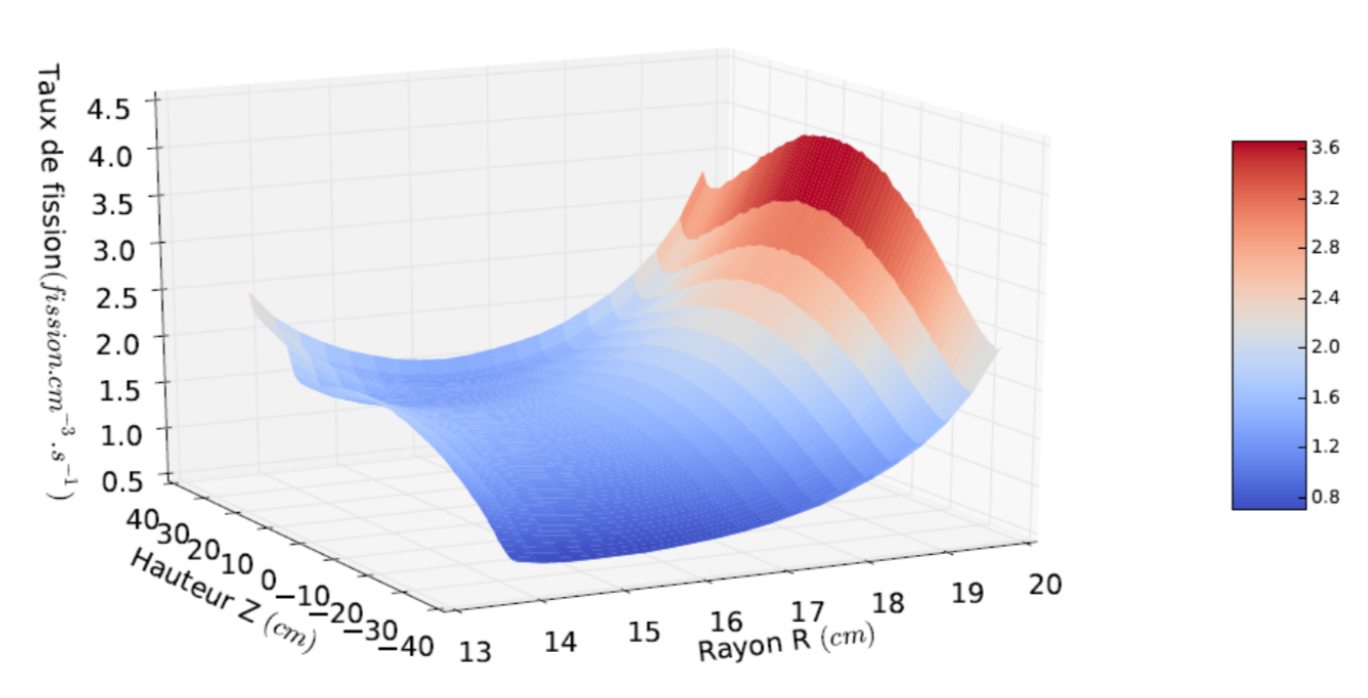
\includegraphics[width=1\textwidth]{images/fissions_dribution_MCNP.png}
\caption[Distribution spatiale des fissions dans le c\oe ur du réacteur de l'ILL]{Distribution spatiale des fissions dans le c\oe ur du réacteur de l'ILL. Ces simulations ont été effectuées avec MCNP.}
\label{fig:fissions_dribution_MCNP}

\end{figure}

}

Le vertex d'interaction quant à lui est tiré dans une large zone incluant tout le détecteur interne: Target, Gamma Catcher, y compris les parois en acrylique et la structure porteuse. Pour prendre en compte les différents matériaux qui composent le détecteur, le volume d'interaction est choisi à chaque événement neutrino avec une probabilité qui prend en compte la densité de protons. Le vertex est ensuite tiré uniformément dans le volume sélectionné. Une dernière condition est appliquée pour considérer la diminution du flux avec la distance. En effet le flux neutrino diminue en $1/L^2$, alors un nombre aléatoire est généré et si sa valeur est inférieure à $1/L^2$, le vertex est accepté.
%
%\begin{itemize}
%    \item Simulation du c\oe ur
%    \item Tirage aléatoire /spectre position
%\end{itemize}

\subsection{Prédiction des spectres neutrino à l'émission}
\label{sec:nu_emission}

Bien que l'analyse d'oscillations décrite dans le Chapitre \ref{chap:chapitre_stat} laisse la prédiction des spectres neutrino complètement libre, une estimation précise de la forme des spectres facilite la convergence  de l'ajustement de la simulation et pose les bases de la mesure absolue.\\

La prédiction des spectres à l'émission est déterminée par l'ensemble des produits de fission qui émettent des neutrinos par décroissante beta. L'évolution de la teneur en combustible du c\oe ur de l'ILL pendant un cycle à pleine puissance nominale a été simulée à l'aide du code : FISPACT \cite{Sublet:2017mbt}. À cause de la courte durée de chaque cycle et du fort enrichissement du combustible en $\ce{^{235}U}$ ($\sim 93 \%$), la production de $\ce{^{239}Pu}$ ne s'élève qu'à $0.7 \%$ en moyenne sur tout le cycle. Sa contribution à la prédiction du spectre d'antineutrinos est donc négligeable. C'est pourquoi la prédiction d'un spectre pur $\ce{^{235}U}$ fournie par Huber \cite{Huber:2011wv} a été utilisée en première approximation.\\

\afterpage{

% corrections_comparison_for_each_bin.pdf
\begin{figure}[h!]
\centering
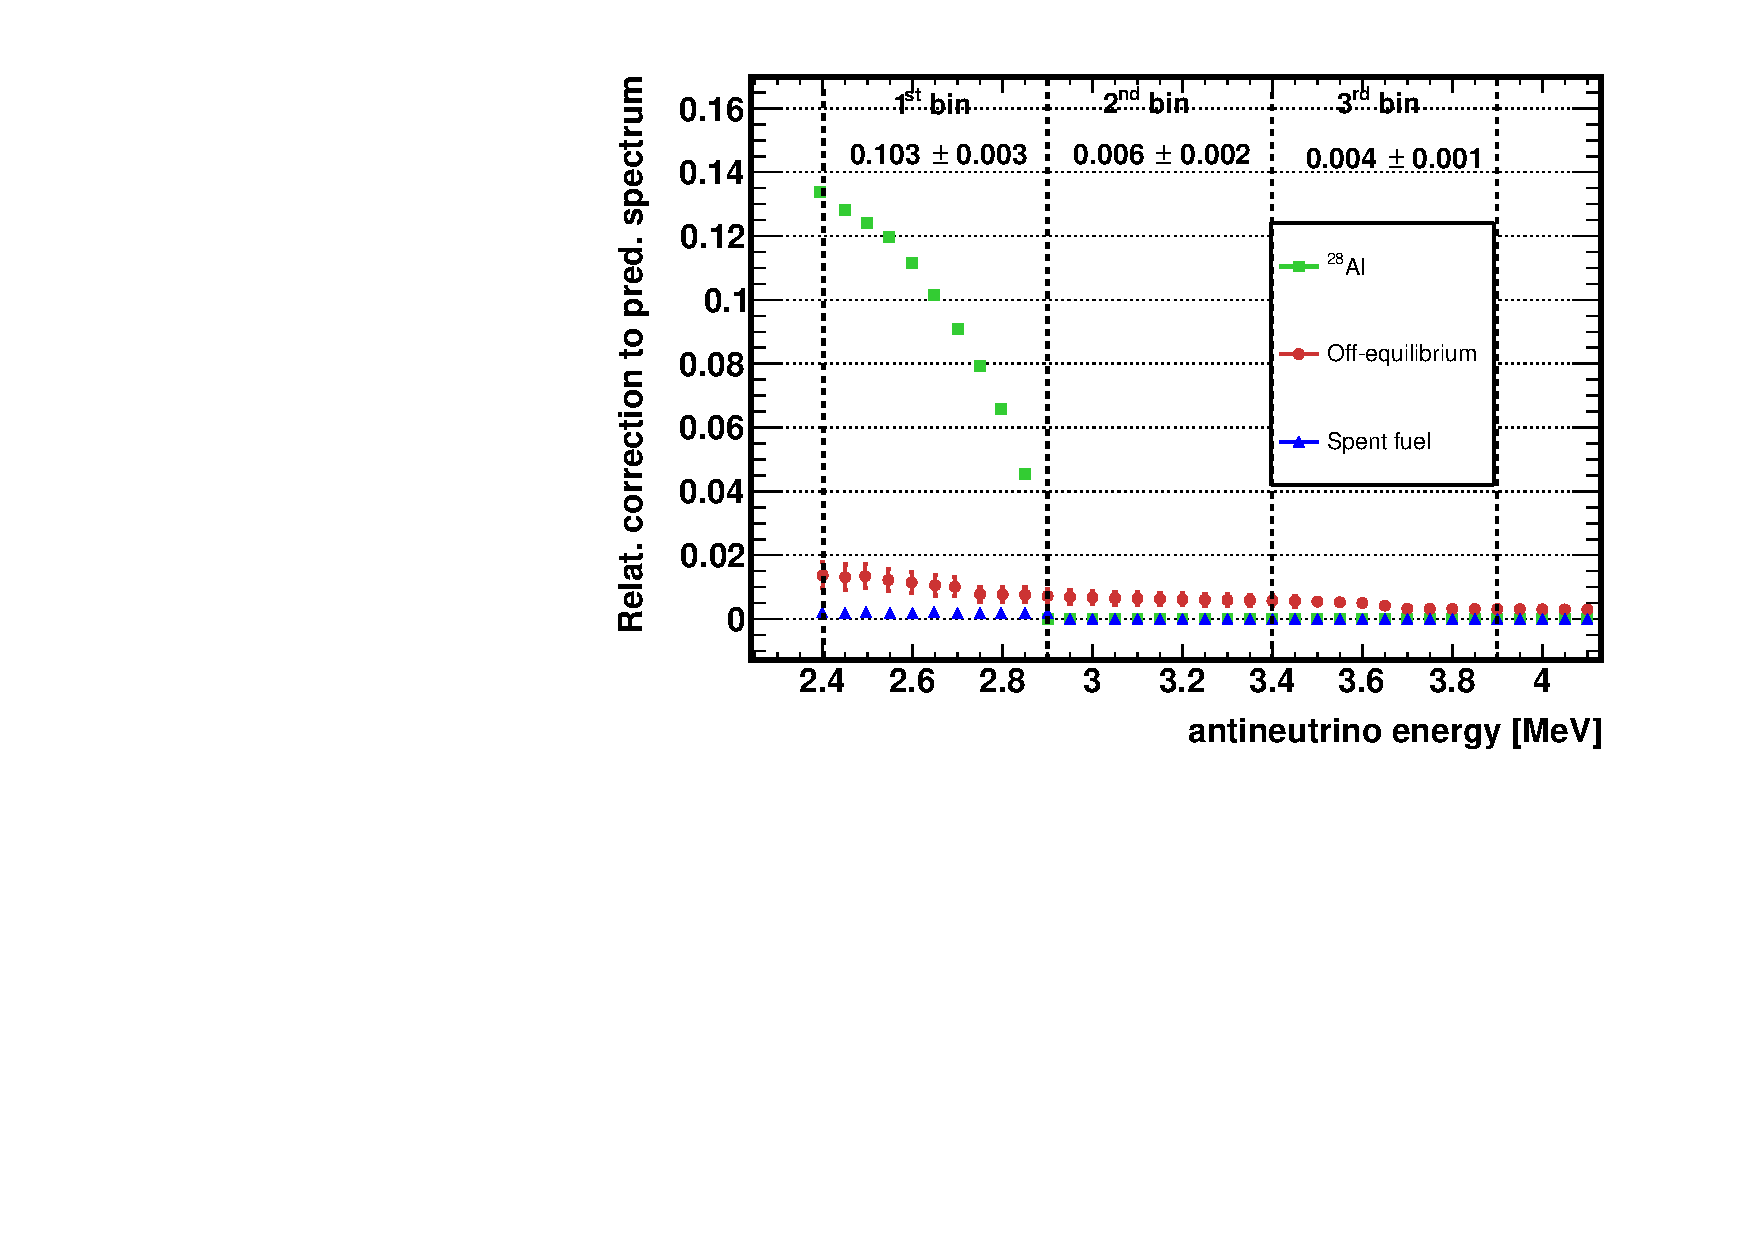
\includegraphics[width=0.8\textwidth]{images/corrections_comparison_for_each_bin.pdf}
\caption[Évolution des différents facteurs de corrections sur les prédictions de spectres antineutrino d'Huber]{Évolution des différents facteurs de corrections sur les prédictions de spectres antineutrino d'Huber: effets hors équilibre (rouge), antineutrinos résiduels (bleu) et la contribution d’antineutrinos issus de la décroissance beta de l'$\ce{^{28}Al}$ (vert). Les lignes verticales en pointillé représentent les premiers bins en énergie qui sont sollicités lors de l'analyse des oscillations. (source : \cite{docdb905})}
\label{fig:correction_fissions_dribution_MCNP}

\end{figure}


}

Bien que ce modèle soit issu de la conversion des spectres beta de fission mesurés auprès du même réacteur à l'ILL dans les années 80 \cite{Schreckenbach:1985ep, VonFeilitzsch:1982jw}, plusieurs corrections doivent être appliquées. \'Etant donné que les mesures de spectres d'électrons issus de la décroissance beta d'$\ce{^{235}U}$ ont été effectuée en irradiant un échantillon pendant environ 12 h \cite{Schreckenbach:1985ep}, les produits de fission qui ont une durée de vie supérieure ou équivalente à 12h ne sont pas pris en compte. Leur contribution doit donc être estimée pour corriger la prédiction des spectres neutrino sur des cycles de 50 jours. Cette correction est appelée : \og corrections hors équilibre \fg{} ou \og \textit{off-equilibrium corrections}\fg{}. De plus une fois que le réacteur est arrêté, le combustible usé est transféré dans la piscine de stockage juste au-dessus du détecteur \textsc{Stereo}. Bien que ce dernier soit refroidi, les mêmes produits de fission à long temps de vie (> 12h) continuent à émettre des neutrinos pendant les périodes réacteur OFF. Ces deux corrections ont été faites en simulant l'inventaire isotopique au cours d'un cycle avec \texttt{FISPAC} puis en déduisant le spectre d'antineutrinos pour chaque élément avec le code \texttt{BESTIOLE}\footnote{Code de calcul des spectres beta de tous les noyaux répertoriés dans la base de données ENSDF, développé pendant la thèse de T. Mueller \cite{Mueller:2010mja}}. Les corrections sont appliquées à partir des spectres antineutrinos prédits par Huber ($S^H(E_\nu)$) en considérant des cycles de 50 jours:

\begin{equation}
\label{eq:corrected_huber_spectrum}
    S^H(E_\nu) \rightarrow S^H(E_\nu) \times \left( 1 + \delta^\textrm{Off-equilibrium} (E_\nu) + \delta^\textrm{Combustible usé} (E_\nu) \right),
\end{equation}

\bigbreak

\noindent
où $\delta^\textrm{Off-equilibrium}$ et $\delta^\textrm{Combustibles usés}$ sont les corrections relatives causées par les effets hors équilibre et le stockage des combustibles usés respectivement. Ces facteurs de correction sont évalués en fonction de l'énergie neutrino sur la figure \ref{fig:correction_fissions_dribution_MCNP}.\\

Ces corrections affectent principalement les trois premiers bins en énergie du spectre positron utilisé pour l'analyse des oscillations. En effet, la contribution des produits de fission à longue durée de vie est essentiellement dominée par trois isotopes qui ont un spectre beta avec un \textit{end-point} entre 3 et $\SI{3.5}{MeV}$: $\ce{^{144}Pr}$, $\ce{^{92}Y}$ et $\ce{^{106}Rh}$. Comparées aux réacteurs commerciaux, les corrections invoquées pour \textsc{Stereo} sont plus faibles à cause de la courte période des cycles à l'ILL qui limite l'accumulation de ces isotopes à longs temps de vie.\\

La troisième correction qui est présentée sur la figure \ref{fig:fissions_dribution_MCNP} est due aux neutrinos produits par l'$\ce{^{28}Al}$. La matrice en aluminium du c\oe ur est soumise à un important flux de neutrons et après capture neutronique ($\ce{^{27}Al(n,\gamma)^{28}Al}$), l'$\ce{^{28}Al}$ décroit par transition beta avec un \textit{end-point} à $\SI{2.86}{MeV}$. Sa contribution au premier bin en énergie de \textsc{Stereo} est estimée à $(10.3 \pm 0.3) \%$.\\




% Pour résumer, la prédiction du spectre d'antineutrinos à l'émission du c\oe ur de l'ILL est construite à partir du modèle d'Huber pur $\ce{^{235}U}$, puis corrigé de la contribution de l'$\ce{^{28}Al}$, des combustibles usés, et des effets hors équilibre.



\bigbreak

%\begin{itemize}
%    \item Prédiction des spectres à l'émission (isotopes / discussion branches interdites) Huber Muller / Schreckenbach ?
%    \item Sources neutrinos annexes (Al matrice, combustible usé)
%%    \item Relation energie neutrino / energie positron
%%    \item Sections efficaces IBD en fonction energie
%%    \item Spectre en énergie
%\end{itemize}

\bigbreak

\subsection{Prédiction des spectres neutrino à l'interaction}
\label{sec:nu_interaction}

Le modèle de spectre d'antineutrinos détectés $M(E_\nu)$ est établi par $S^\textrm{tot}(E_\nu)$, la prédiction corrigée d'Huber pure $\ce{^{235}U}$ (Équation \ref{eq:corrected_huber_spectrum} + corrections figure \ref{fig:fissions_dribution_MCNP}) multipliée par la section efficace d'interaction IBD $\sigma_{V-A}(E_\nu)$:

\begin{equation}
    M(E_\nu) = S^\textrm{tot}(E_\nu) \times \sigma_{V-A}(E_\nu)
\end{equation}

\bigbreak

\afterpage{

% detected_spectrum.pdf
\begin{figure}[h!]
\centering
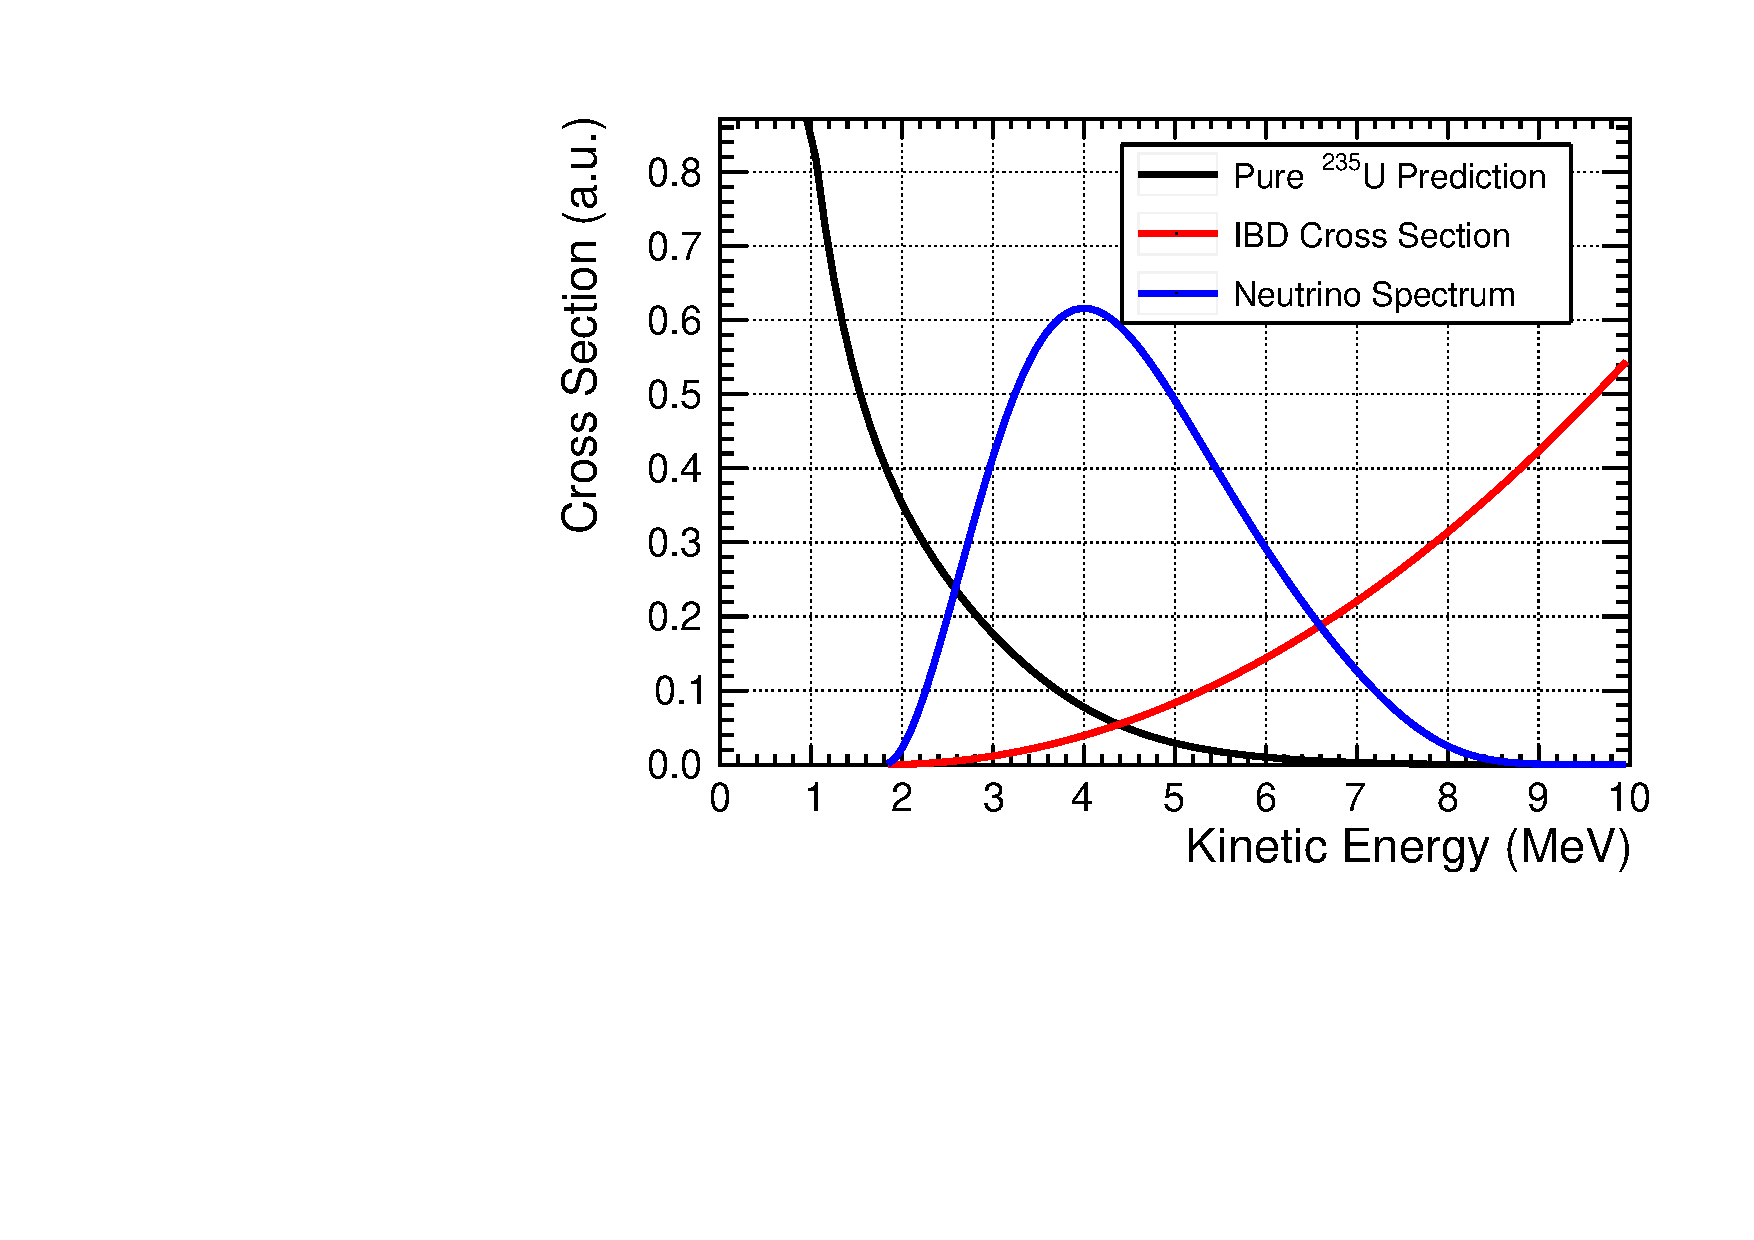
\includegraphics[width=0.8\textwidth]{images/detected_spectrum.pdf}
\caption[Construction des spectres positrons dans \textsc{Stereo}]{Construction des spectres positrons dans \textsc{Stereo}. La courbe noire représente le spectre antineutrino pur $\ce{^{235}U}$ prédit par Huber, en rouge la section efficace IBD en fonction de l'énergie du neutrino, en bleu le spectre d'antineutrinos qui interagissent dans \textsc{Stereo}.}
\label{fig:detected_spectrum.pdf}

\end{figure}


}

où $\sigma_{V-A}(E_\nu)$ est donnée par le modèle à basse énergie de Vogel \cite{Vogel:1983hi}. En pratique, le spectre antineutrino est déduit de l'énergie du positron via la relation : $E_\nu \simeq E_e + M_n - M_p = E_e + \SI{1.806}{MeV}$ où $M_n$ et $M_p$ sont la masse du neutron et celle proton respectivement. Alors, $\sigma_{V-A}(E_e)$ peut être écrit sous la forme:

\begin{equation}
    \sigma_{V-A}(E_e) = \frac{2\pi^2\hbar^3}{m_e^5c^7f\tau_n} p_e E_e \left(1 + \delta_\textrm{rec} + \delta_\textrm{WM} + \delta_\textrm{rad} \right),
\end{equation}

avec $m_e$ et $p_e$ la masse et l'impulsion du positron respectivement, $\tau_n$ le temps de vie du neutron, $f$ le facteur d'espace de phase du neutron \cite{Wilkinson:1998hx}, $\delta_\textrm{rec}$ le facteur de correction pour considérer le recul du proton, $\delta_\textrm{WM}$ pour le \textit{Weak-Magnetism}, et $\delta_\textrm{rad}$ pour les corrections radiatives. À titre d'illustration, les spectres $S^\textrm{tot}(E_\nu)$, $\sigma_{V-A}(E_\nu)$, $M(E_\nu)$ et $M(E_e)$ sont représentés sur la figure \ref{fig:detected_spectrum.pdf}.\\

Ainsi, l'énergie des neutrinos dans la simulation est attribuée en tirant aléatoirement dans le spectre $M(E_\nu)$. À chaque événement IBD, un positron et un neutron sont générés dans \textsc{Geant4}. L'énergie du positron $E_e$ est directement déduite de celle du neutrino choisi $E_\nu$, et l'impulsion du neutron est choisie indépendamment suivant la formule issue de \cite{Vogel:1999zy}\footnote{Pour obtenir l'expression de l'énergie cinétique du neutron, un développement au premier ordre en $1/M_p$ de $E_e$ est nécessaire.} :

\begin{equation}
\label{eq:e_neutron_IBD}
    E_n \simeq \frac{E_\nu E_e + ((E_\nu - E_e)^2 - m_e^2)/2}{M_p}.
\end{equation}

\bigbreak

L'énergie cinétique du neutron $E_n$ reste toujours très faible devant l'énergie du positron ($E_n \sim \SI{20}{keV} \ll E_e$), et dépend de $E_e$ dans l'Equation \ref{eq:e_neutron_IBD}. De plus, afin de reproduire au mieux les effets de bord sur l'efficacité de détection, l'angle d'émission des deux particules est injecté selon les prédiction de Vogel et Beacom \cite{Vogel:1999zy}.

%\begin{itemize}
%    \item Relation energie neutrino / energie positron
%    \item Sections efficaces IBD en fonction énergie
%    \item Spectre en énergie
%\end{itemize}

\bigbreak

\subsection{Contrôle de l'efficacité de détection}
\label{sec:control_eff_det}

Un des objectifs de \textsc{Stereo} est de tester l'anomalie de flux. Cette mesure requiert une grande précision sur le contrôle de l'efficacité de détection, sur la prédiction des spectres ainsi que sur l'acceptance géométrique. La quantité de neutrinos détectés par jour dans \textsc{Stereo} peut être exprimée en fonction du flux émis par le réacteur :

\begin{equation}
\label{eq:nu_det_eff_def}
    \phi_\nu^{\textrm{det}} = \phi_\nu^{\textrm{em}} \times \int_{E_\nu} dE_\nu S^\textrm{tot}(E_\nu) \sigma_{V-A}(E_\nu) \int_{V_c} d\overrightarrow{r_c} \rho_c(\overrightarrow{r_c}) \int_{V_d} d\overrightarrow{r_d} \rho_d(\overrightarrow{r_d}) \times \frac{\varepsilon_d(\overrightarrow{r_d}, E_\nu)}{4\pi (\overrightarrow{r_d} - \overrightarrow{r_c})^2},
\end{equation}

\bigbreak

où $\phi_\nu^{\textrm{em}}$ est le flux d'antineutrinos émis par le réacteur (défini dans le Chapitre \ref{chap:chapitre_2}, Éq. \ref{eq:phi_nu_em}), $V_c$ représente le volume du c\oe ur et $\rho_c(\overline{r_c})$ la densité de fission locale; et $V_d$ le volume de détection où $\rho_d$ est la densité de protons en $\overrightarrow{r_d}$. Notons que d'après cette définition, les intégrales de $\rho_c$ sur le volume du c\oe ur $V_c$ et $S^\textrm{tot}(E_\nu)$ sur le spectre neutrino sont égales à 1, car c'est $\phi_\nu^{\textrm{em}}$ qui contient la normalisation du nombre de neutrinos émis. L'efficacité de détection des neutrinos est prise en compte par $\varepsilon_d$ qui représente la quantité de neutrinos qui passent les coupures de sélection des paires Prompt-Retardé (énergie, fenêtre Prompt-Retardé, PSD...) à $\overrightarrow{r_d}$ avec une énergie $E_\nu$.\\

Pour calculer $\phi_\nu^{\textrm{det}}$, il est judicieux d'introduire l'acceptance géométrique $\tau_\nu$ qui exprime la quantité de neutrinos qui interagissent autour du détecteur sans considérer l'efficacité de détection $\varepsilon_d$:

\begin{equation}
\begin{gathered}
    \delta \tau_\nu(E_\nu,\overrightarrow{r_c},\overrightarrow{r_d}) \doteq dE_\nu d\overrightarrow{r_c} d\overrightarrow{r_d} \frac{\rho_c(\overrightarrow{r_c})\rho_d(\overrightarrow{r_d})}{4\pi (\overrightarrow{r_d} - \overrightarrow{r_c})^2}\textrm{ } S^\textrm{tot}(E_\nu) \sigma_{V-A}(E_\nu).\\
    \textrm{donc : } \tau_\nu = \int_{E_\nu} dE_\nu \int_{V_c} d\overrightarrow{r_c} \int_{V_d} d\overrightarrow{r_d} \left\{ \frac{\rho_c(\overrightarrow{r_c})\rho_d(\overrightarrow{r_d})}{4 \pi (\overrightarrow{r_d} - \overrightarrow{r_c})^2} \textrm{ } S^\textrm{tot}(E_\nu) \sigma_{V-A}(E_\nu) \right\} .
\end{gathered}
\end{equation}

\bigbreak

\afterpage{
%tau_nu.png

\begin{figure}[h!]
\centering
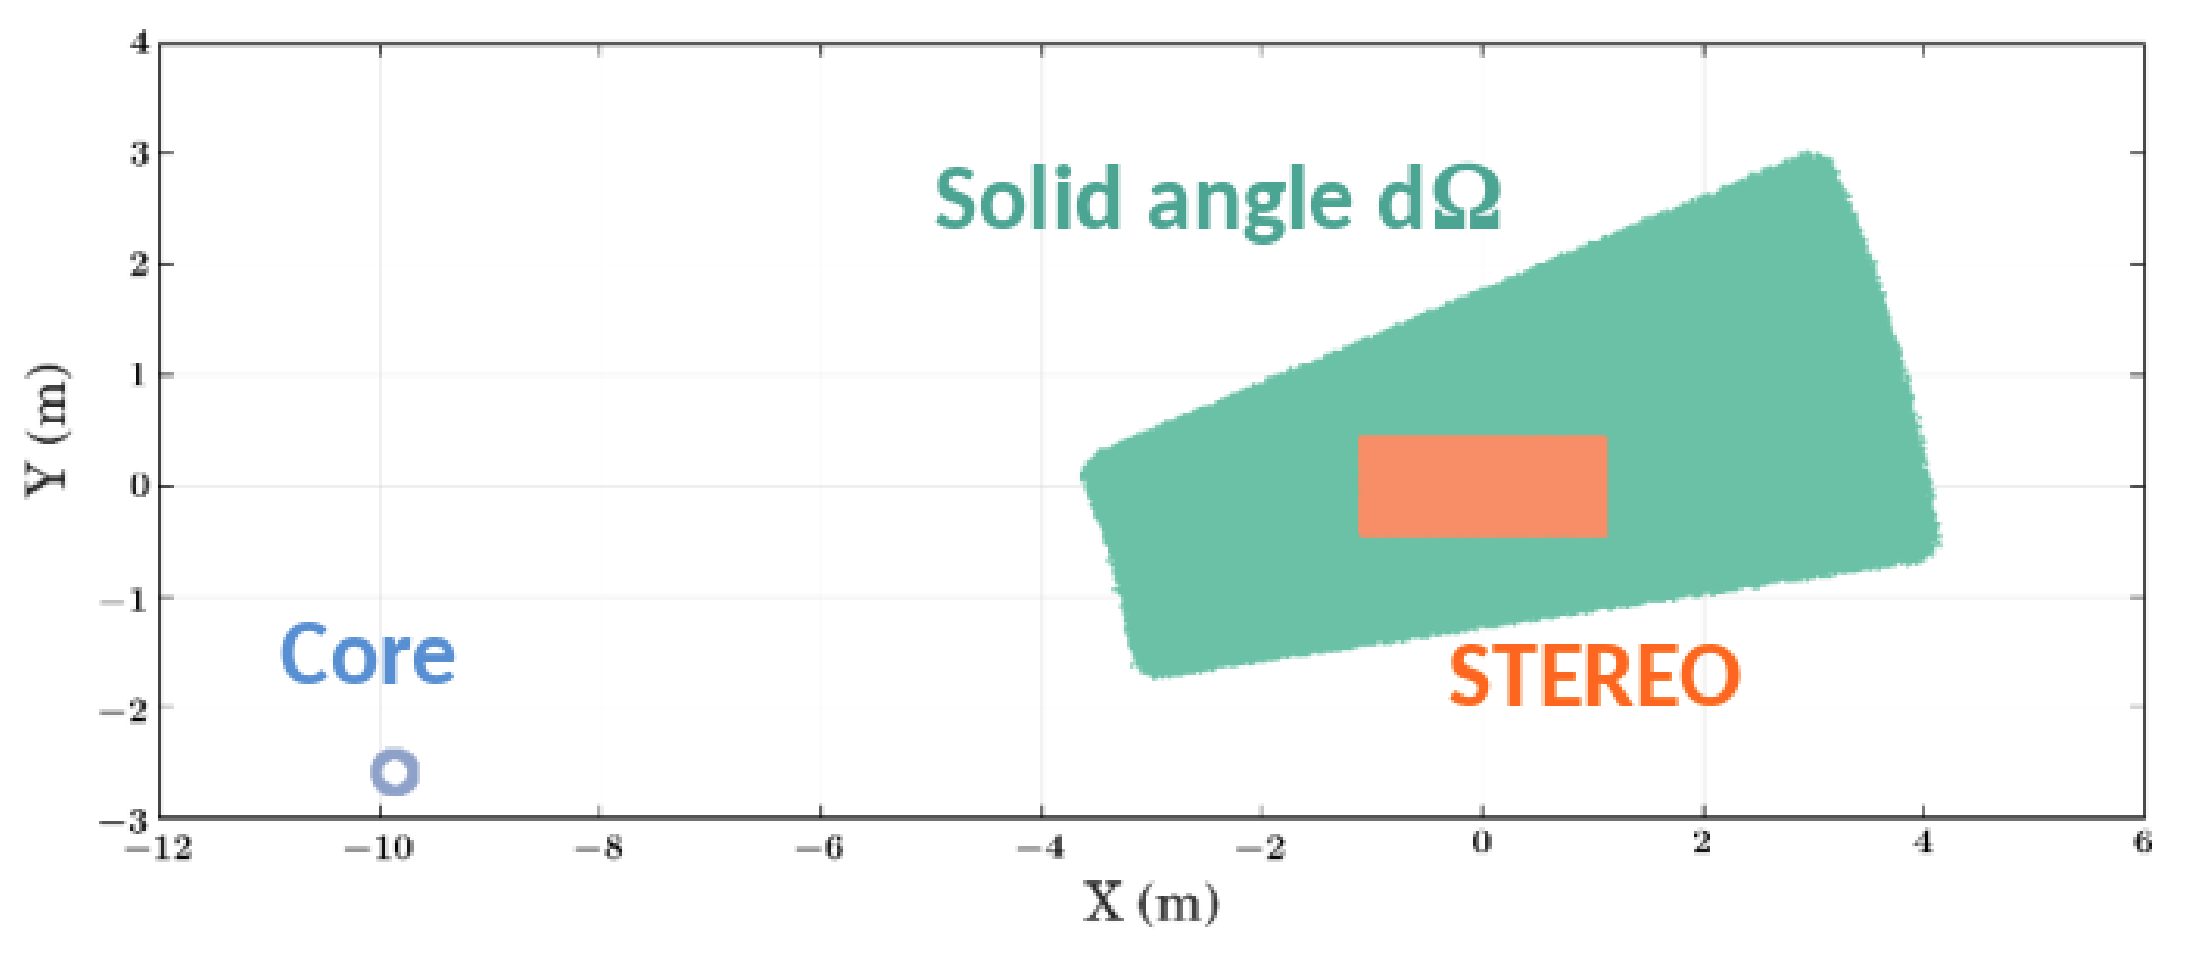
\includegraphics[width=1\textwidth]{images/tau_nu.png}
\caption[Estimation de l'acceptance géométrique de \textsc{Stereo}]{Estimation de l'acceptance géométrique de \textsc{Stereo}. Les vertex d'émission (bleu) et d'interaction (vert et orange) des neutrinos sont tirés pour le calcul de l'acceptance géométrique. La zone orange représente l'emplacement du détecteur. (source : \cite{docdb711})}
\label{fig:tau_nu.png}

\end{figure}

}

En d'autres mots, $\tau_\nu$ exprime la probabilité qu'un neutrino interagisse. $\tau_\nu$ est estimé numériquement par échantillonnage de traces neutrino. Comme décrit dans la section \ref{seq:mc_nu_vertex_em_int}, les vertex d'émission sont tirés suivant le spectre $S^\textrm{tot}(E_\nu)$ et un modèle de distribution spatiale des fissions $\rho^i_c(\overrightarrow{r_c})$, tandis que les points d'interaction sont choisis uniformément dans un large volume incluant le détecteur. Ce volume choisi est décrit par un angle solide $\Delta \Omega$ et une plage de distances de propagation $\Delta r$. Chaque trace neutrino $i$ est pondérée par la probabilité d'interaction $\omega_i$. La figure \ref{fig:tau_nu.png} représente le volume de tirage et le volume couvert. L'acceptance géométrique est calculée en générant un grand nombre de traces neutrino $N$:

\begin{equation}
\label{eq:numerical_geom_acc}
    \tau_\nu = \frac{\sum_{i=1}^{N} \omega_i}{\sum_{i=1}^{N} 1} \times \frac{\Delta \Omega}{4\pi} = \frac{\sum_{i=1}^{N} \left\{ \sigma_{V-A}(E_\nu) \rho^i_d(\overrightarrow{r_d}) \right\} }{N} \times \Delta r \frac{\Delta \Omega}{4\pi},
\end{equation}

\bigbreak

Une fois que $\tau_\nu$ est défini, la densité de probabilité d'interaction sachant $E_\nu$, $\overrightarrow{r_c}$ et $\overrightarrow{r_d}$ peut être construite en normalisant:

\begin{equation}
\begin{gathered}
    \frac{\rho_c^*(\overrightarrow{r_c})\rho_d^*(\overrightarrow{r_d})}{4\pi (\overrightarrow{r_d}^* - \overrightarrow{r_c}^*)^2}\textrm{ } S^{\textrm{tot}*}(E_\nu) \sigma_{V-A}^*(E_\nu) \doteq \frac{\frac{\rho_c(\overrightarrow{r_c})\rho_d(\overrightarrow{r_d})}{4\pi (\overrightarrow{r_d} - \overrightarrow{r_c})^2} \textrm{ } S^\textrm{tot}(E_\nu) \sigma_{V-A}(E_\nu)}{\tau_\nu},\\
    \textrm{tel que : } \int_{E_\nu} dE_\nu \int_{V_c} d\overrightarrow{r_c} \int_{V_d} d\overrightarrow{r_d} \left\{ \frac{\rho_c^*(\overrightarrow{r_c})\rho_d^*(\overrightarrow{r_d})}{4\pi (\overrightarrow{r_d}^* - \overrightarrow{r_c}^*)^2}\textrm{ } S^{\textrm{tot}*}(E_\nu) \sigma_{V-A}^*(E_\nu) \right\} = 1.
\end{gathered}
\end{equation}

\bigbreak

Cette distinction permet de séparer les considérations d'acceptance géométrique de l'efficacité de détection des coupures de sélection dans l'Équation (\ref{eq:nu_det_eff_def}). En effet, $\phi_\nu^{\textrm{det}}$ peut maintenant être exprimée en fonction d'une efficacité de détection totale $\varepsilon_d^{\textrm{tot}}$:

\begin{equation}
\label{eq:phi_nu_simple}
    \phi_\nu^{\textrm{det}} = \phi_\nu^{\textrm{em}} \times \tau_\nu \times \varepsilon_d^{\textrm{tot}},
\end{equation}

\bigbreak

où $\varepsilon_d^{\textrm{tot}}$ est définie comme la moyenne de $\varepsilon_d$ pondérée suivant la densité de probabilité d'interaction\footnote{La moyenne d'une variable $x$ distribuée suivant une distribution de probabilité $P(x)$ est $\bar{x} = \int xP(x) dx$.} :

\begin{equation}
\label{eq:def_detection_eff}
    \varepsilon_d^{\textrm{tot}} = \int_{E_\nu} dE_\nu \int_{V_c} d\overrightarrow{r_c} \int_{V_d} d\overrightarrow{r_d} \left\{ \frac{\rho_c^*(\overrightarrow{r_c})\rho_d^*(\overrightarrow{r_d})}{4\pi (\overrightarrow{r_d}^* - \overrightarrow{r_c}^*)^2}\textrm{ } S^{\textrm{tot}*}(E_\nu) \sigma_{V-A}^*(E_\nu) \right\} \varepsilon_d(\overrightarrow{r_d}, E_\nu).
\end{equation}

\bigbreak

L'efficacité totale de détection est estimée avec les simulations Géant4. Seules les traces neutrinos qui ont un poids d'acceptance géométrique $\omega_i$ non nul  (cf. Équation \ref{eq:numerical_geom_acc}) sont envoyés dans la simulation. En pratique, plusieurs milliers de réactions IBD sont injectés dans \textsc{Geant4}. $\varepsilon_d^{\textrm{tot}}$ est obtenu en calculant la fraction d'événements simulés qui ont passé l'ensemble des coupures topologiques imposées dans les données. Ces coupures sont explicitées dans la section \ref{sec:cuts}.

\bigbreak

\subsection{Pondérations et motifs d'oscillation}
\label{sec:building_oscillation}

Pour tester différentes hypothèses sur la forme des spectres, un jeu de données simulées adéquat doit être comparé aux spectres neutrinos mesurés avec \textsc{Stereo}. Pour des raisons d'optimisation de temps de calcul, un seul jeu de données neutrino est simulé avec un spectre plat. Les spectres en énergie neutrino sont appliqués en aval en construisant des séries d'histogrammes en énergie positron (ou énergie visible) pour chaque hypothèse à tester. En pratique, ces histogrammes ont les mêmes dimensions que ceux des données \textsc{Stereo} (bornes et binning) et sont remplis en appliquant un poids $\omega$ à chaque événement neutrino simulé:

\begin{equation}
    w \doteq S^\textrm{tot}(E_\nu) \sigma_{V-A}(E_\nu)
\end{equation}

\bigbreak

\afterpage{
%bending_factor.pdf

\begin{figure}[h!]
\centering
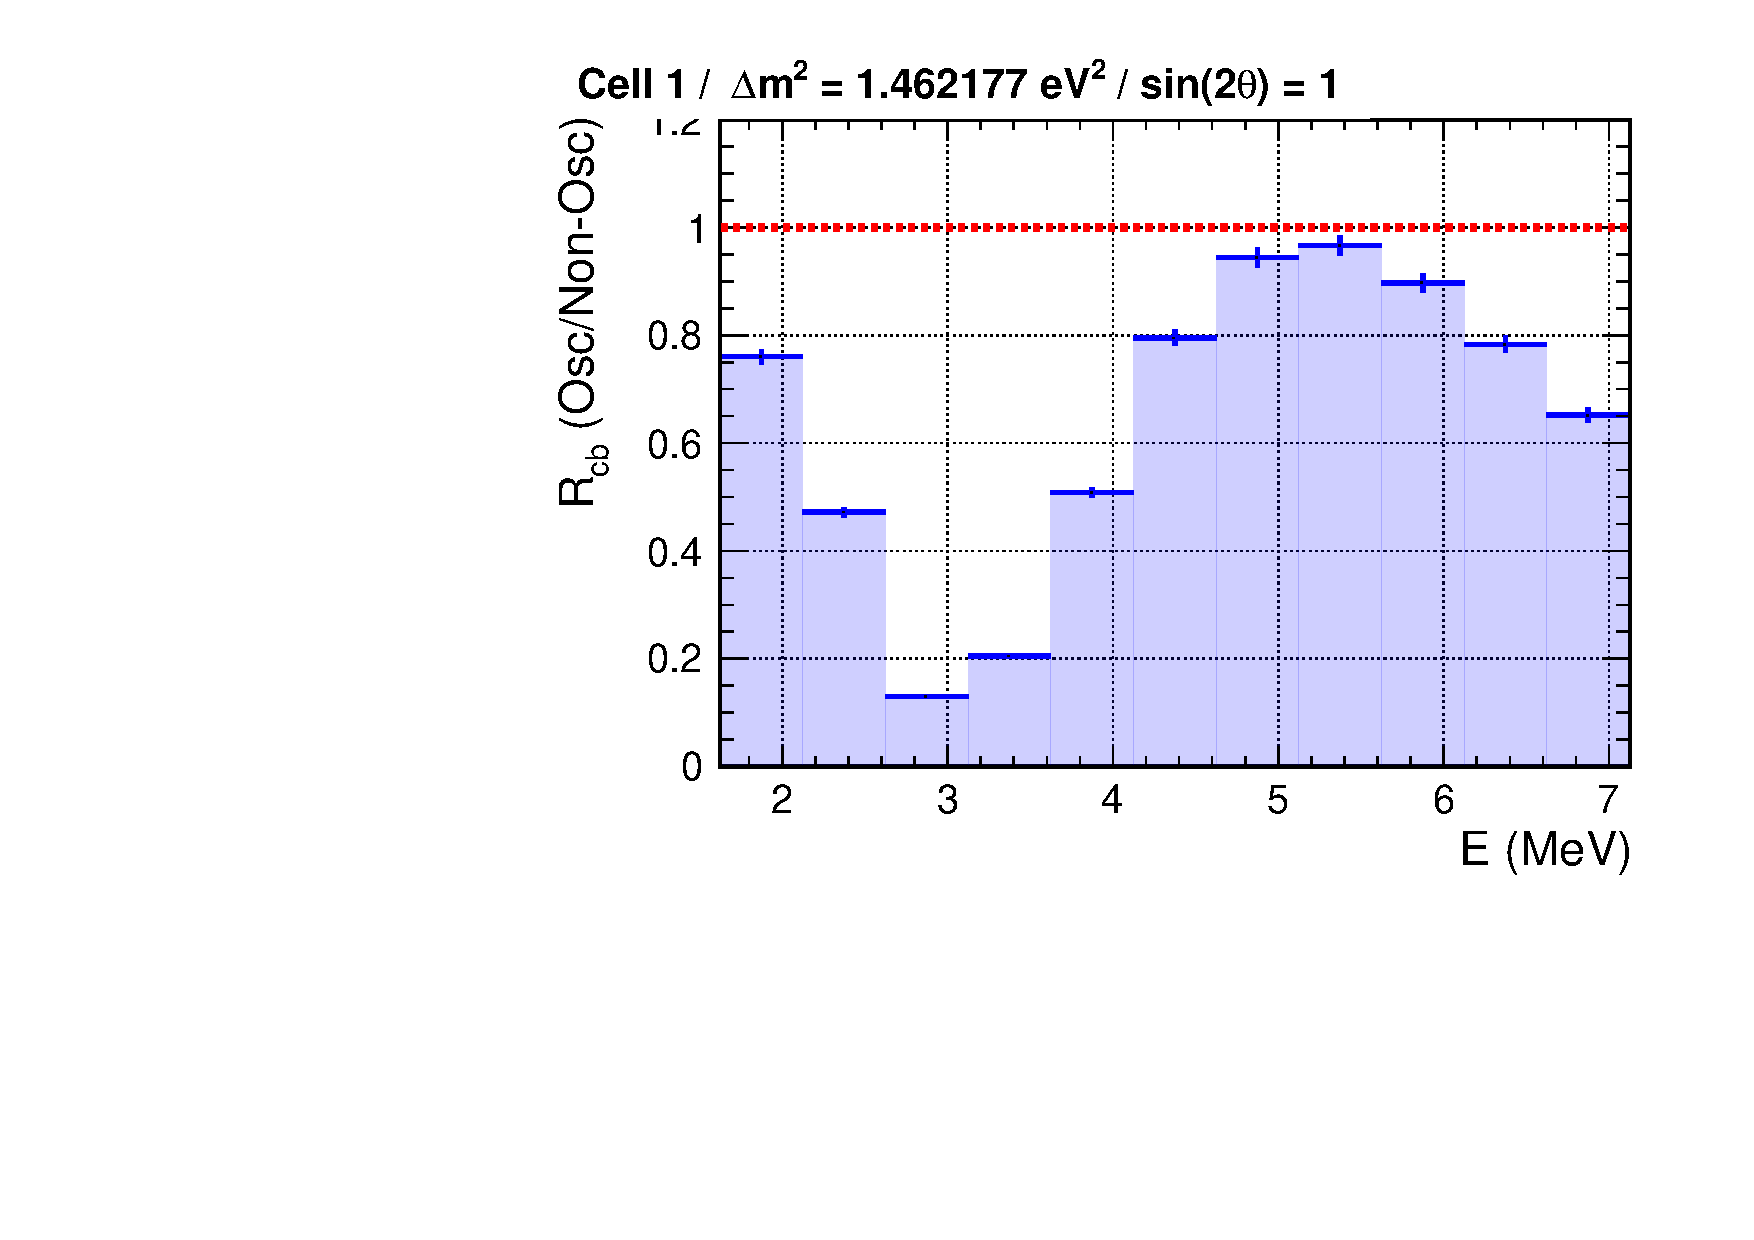
\includegraphics[width=1\textwidth]{images/bending_factor.pdf}
\caption[Rapport des spectres positron oscillé/non-oscillé]{Rapport des spectres positron oscillé/non-oscillé : $R_{cb} = M_{cb}^\textrm{osc}/M_{cb}^\textrm{non-osc}$. La ligne rouge représente le cas sans oscillation.}
\label{fig:bending_factor.pdf}

\end{figure}

}

Dans le cadre de la génération des contours de sensibilité, les distorsions sur les spectres de chaque cellule sont déterminées par l'amplitude et la fréquence d'oscillation : $\textrm{sin}^2(2\theta_{14})$ et $\Delta m_{14}^2$ respectivement. La probabilité $P_{\overline{\nu}_e \rightarrow \overline{\nu}_e}$ intervient dans l'expression de $w$ :

\begin{equation}
    w \rightarrow w \times P_{\overline{\nu}_e \rightarrow \overline{\nu}_e} (E_\nu, \textrm{sin}^2(2\theta_{14}), \Delta m_{14}^2).
\end{equation}

\bigbreak

Dans l'analyse d'oscillations, les hypothèses à tester sont réparties sur une grille ($\Delta m_{14}^2; \textrm{sin}^2(2\theta_{14})$) avec une échelle logarithmique. En pratique $100 \times 100$ hypothèses d'oscillations sont testés. Encore pour des raisons de réduction de temps de calcul et d'espace disque, seuls les histogrammes en énergie positron avec $\textrm{sin}^2(2\theta_{14}) = 1$ sont stockés. Ainsi à chaque $\Delta m_{14}^2$, seul le rapport des histogrammes oscillé sur non-oscillé est enregistré:

\begin{equation}
R_{cb}(\Delta m_{14}^2) = \frac{M_{cb}^\textrm{osc} \left(\Delta m_{14}^2, \textrm{sin}^2(2\theta_{14}) = 1\right)}{M_{cb}^\textrm{non-osc}}
\end{equation}

\bigbreak

où $M_{cb}$ est le bin $b$ de l'histogramme représentant le spectre en énergie positron dans la cellule $c$. Un exemple de rapport de spectres est présenté sur la figure \ref{fig:bending_factor.pdf}. Un scénario d'oscillation particulier ($\Delta m_{14}^2; \textrm{sin}^2(2\theta_{14})$) est ensuite recouvré à l'aide de $R_{cb}(\Delta m_{14}^2)$ :

\begin{equation}
    M_{cb}^\textrm{osc} \left(\Delta m_{14}^2, \textrm{sin}^2(2\theta_{14})\right) = M_{cb}^\textrm{non-osc} \times \left[1 - \textrm{sin}^2(2\theta_{14}) \left( 1 - R_{cb}(\Delta m_{14}^2) \right)\right].
\end{equation}

\bigbreak

Ce sont ces $M_{cb}^\textrm{osc}$ qui sont comparés avec les données mesurées pour l'analyse d'oscillation. Cette étude est présentée en détail dans le Chapitre \ref{chap:chapitre_stat}.

